\documentclass[a4j,xelatex,ja=standard]{bxjsarticle}
\RequirePackage[l2tabu, orthodox]{nag}
\usepackage[all, warning]{onlyamsmath}
\usepackage{fontspec}
\usepackage{amsmath}
\usepackage[upgreek]{txgreeks}
% \setpagelayout{left=20mm,top=15mm,right=20mm,bottom=15mm,nohead}
%\usepackage{xltxtra}
%\usepackage{zxjatype}
\setmainfont{Noto Serif CJK JP}
\setsansfont{Noto Sans CJK JP}
\setmonofont{Noto Sans Mono CJK JP}
\setCJKmainfont{Noto Serif CJK JP}
\setCJKsansfont{Noto Sans CJK JP}
\setCJKmonofont{Noto Sans Mono CJK JP}
% \pagestyle{empty}
%\setlength{\topmargin}{10mm}
%\addtolength{\topmargin}{-1in}

% \def\tightlist{\itemsep1pt\parskip0pt\parsep0pt}

\title{Understanding the Masking-Shadowing Function in Microfacet-Based BRDFs (JCGT 2014)}
\author{Eric Heitz \\ INRIA ; CNRS ; Univ. Grenoble Alpes}

\begin{document}

\maketitle

\section{まえがき(Introduction)}

マイクロファセット理論は元々、表面上の散乱を研究するために光物性(optical physics)の分野で開発された。グラフィクス界隈では物理ベースのBRDFを導入するために使われ、こんにちの3DCGには欠かせない技術となっている。2012年と2013年のSIGGRAPHにはマイクロファセット理論を扱うコースもあり、そこではアーティストによる調整のしやすさや計算の効率性などについても議論されている。マイクロファセットは、要素の組み合わせの数だけ可能性が存在するため、今なお盛んな分野である。しかし、要素の適切な選び方が明白でないことままあるため、混乱の主な原因になっている。

\paragraph{この文書で取り上げること(What This Document Is About)}

この文書では、マイクロファセットベースのBRDFにおけるmasking-shadowing関数の選び方に関する、新しい見方と長年の疑問に対する答えを提供する。

\paragraph{この文書で取り上げないこと(What This Document Is Not About)}

一般的に使われているモデルでのみ議論するのであって、新しいBRDFモデルを提案したりはしない。理解を深めるためにモデルについての背景知識を提供するのが目的であって、他のモデルを差し置いて特定のモデルをおすすめしたりはしない。物理パラメータの理解に注力するのであって、すでに使用実績があるからといってその実装や特定のレンダリング技法での使われ方を想定しない。

\paragraph{マイクロファセットモデルにおける"物理ベース"が意味する所(On The Meaning Of "Physically Based" Regarding Microfacet Models)}

物理的モデルとは、解析、説明、挙動の予測が可能であるシステムまたは物理現象の簡略表現である。

マイクロファセット理論において、研究対象であるモデルは、巨視的尺度(macroscopic scale)で見ると平坦な幾何的表面だが、微視的尺度(microscopic scale)で見るとその界面(interface)は荒く、マイクロファセットで構成されている。この表現は、幾何学的表面の界面(geometric surface interface)で発生する散乱現象(scattering events)を説明したり予測したりするときに使われる。

有意義なマイクロファセットモデルは、どれだけマイクロファセットが指定の方向を統計的に見て向いているかを示す法線分布と、どのようにマイクロファセットがマイクロサーフェス上に組織されているかを示すマイクロファセットプロファイルによって説明される。このような有意義なマイクロファセットモデルから導き出された方程式を持つマイクロファセットBRDFは、マイクロサーフェスモデルに基づくことから、まさしく"物理ベース"と呼ばれる。逆に、マイクロサーフェスモデルからBRDFが導けないなら、それは"物理ベース"とは呼ばれない。masking-shadowing関数は、マイクロファセットBRDFの一部で、マイクロファセットが出射方向から(masking)か入射方向から(shadowing)のいずれかから見えている確率を表す。BRDFのときと同様に、マイクロサーフェスモデルから導き出される場合のみ、masking-shadowing関数は"物理ベース"と呼ばれる。

本文書では、マイクロサーフェスモデルが正式にはどのように説明されているか、そこから物理ベースのmasking-shadowing関数がどのように導き出されるかを解説する。これが関連する物理ベースBRDFの導出にどうつながるかも紹介する。

ただし、マイクロファセットモデルは、幾何光学のみを扱う、完全な鏡面および拡散反射、複数回の散乱を考慮しない、といったマイクロサーフェスの光学的な振る舞いに関する仮定に基づく、単なる**モデル**であることに注意すべきである。したがって、"物理ベース"と呼ばれるそれは、現実の物理表面の測定値を正確に予測することができるという意味ではない、ということを頭に入れておく必要がある。仮定したものが間違っていれば、計測データと比較したとき、数学的に厳密な"物理ベース"のそれより経験則的モデルのほうが正確であることも十分にあり得る。

\paragraph{アイデアとOrganization(Ideas and Organization)}

この文書で述べられるアイデアは以下の3つの先行研究に強く影響を受けている:

\begin{itemize}
\item Smithのmasking関数は、コンピュータグラフィクスの文献のなかで最も有名なものの一つである。しかし、この関数が、正しいmasking関数から期待される性質である、可視射影面積(visible projected area)を保持することを保証する性質を持つことを文書の最後に指摘していることはあまり知られていない。

\item Ashikhminらは可視射影面積(visible projected area)が幾何学的表面からマイクロサーフェスに至るまで保存されている量であることを見つけ出した。この知見は、正しく正規化されていることとエネルギーが保存されていることを保証する、正しいmasking項の一般式を導出するために使われた。この導出の最中には、自然とSmithのmasking関数を再発明していた。彼らのmasking項は積分形式で表されており、閉形式を導くことはできない。彼らは数値的に前計算を行い、ルックアップテーブルに格納する方法を取った。

\item Rossらは海面の反射率に関する研究を提案した。ガウス的な荒い表面(Beckmann分布)で海面をモデル化し、Smithのmasking-shadowing関数を組み込んだ正規化済みBRDFを計算した。彼らはガウス的表面ではBRDFの正規化係数とSmithのmasking関数が打ち消し合う?似通った式を持つことを発見した。この性質は計算機処理目的では便利だが、彼らはこれが発生する物理的理由を示さなかった。
\end{itemize}

この文書では、可視射影面積(visible projected area)の保存の観点からこれまでのすべての研究結果を直接導き出せる、統一されたマイクロファセットフレームワークを提案する。

<<各章の概要>>

\section{Masking関数の導出(Derivation of the Masking Function)}

\subsection{表面上での放射輝度の計測(Measuring Radiance on a Surface)}
\label{sec:2.1}

\begin{figure}
    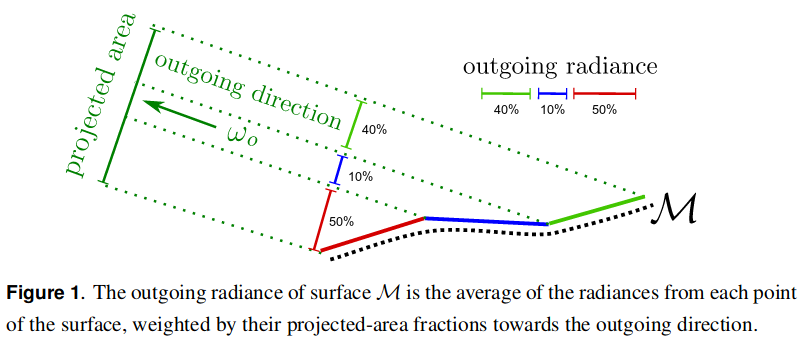
\includegraphics[width=\textwidth]{Figure1.png}
    \caption{}
    \label{fig:1}
\end{figure}

放射輝度(radiance)は立体角からある領域を通過するエネルギー密度で、単位は$\text{W}/\text{sr}/\text{m}^2$である。方向$\boldsymbol{\omega}_o$に出射する面$\mathcal M$の放射輝度$L(\boldsymbol{\omega}_o, \mathcal{M})$は、出射方向に観測される射影面積(projected area)により重み付けされた、表面上の各区間(patch)の中心点$p_m$と出射方向$\boldsymbol{\omega}_o$に対する放射輝度$L(\boldsymbol{\omega}_o, p_m)$を積分したものである。

\begin{equation}
    L(\boldsymbol{\omega}_o, \mathcal{M}) = \frac{\int_{\mathcal M} \text{projected area}(p_m) L(\boldsymbol{\omega}_o, p_m) dp_m}{\int_{\mathcal M} \text{projected area}(p_m) dp_m}
    \label{eq:1}
\end{equation}

出射方向に投影される表面上の各地点での面積は視点依存であり、分母の積分$\int_{\mathcal M} \text{projected area}(p_m) dp_m$は正規化係数である。この正規化係数は式全体が放射輝度を単位とするよう調整している。

\subsection{マイクロファセット統計学(Microfacet Statistics)}

幾何学的表面$\mathcal G$と呼ばれる表面の平面領域を考える。その面積は慣例に従い、$\int_{\mathcal G}dp_g = 1 [\text{m}^2]$である。マイクロファセットモデルは、真の表面がマイクロサーフェス$\mathcal M$と呼ばれるマイクロファセットの集合の形に幾何学的表面からオフセットしたものであると仮定する。正確に言うならば、ジオメトリ$\mathcal G$の法線が$\boldsymbol{\omega}_g$であるとすると、$\mathcal M$は$\boldsymbol{\omega}_g$方向に$\mathcal G$上に投影されたマイクロファセットの点の集合である。マイクロサーフェス$\mathcal M$の各点$p_m$は法線$\boldsymbol{\omega}_m(p_m)$を持つ。すなわち、$\boldsymbol{\omega}_m : \mathcal{M} \rightarrow \Omega$は、マイクロサーフェス上の点からその点の面法線ベクトルへの写像である。このベクトルは$(x_m, y_m, z_m)$として表される。

\begin{figure}
    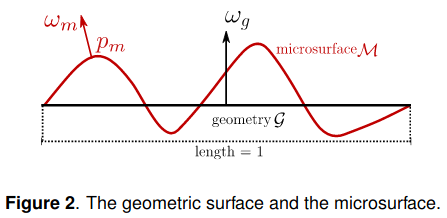
\includegraphics[width=\textwidth]{Figure2.png}
    \caption{}
    \label{fig:2}
\end{figure}

マイクロファセット理論はマイクロサーフェスの散乱の特性を統計学的にモデル化したものである。したがって、数式は空間的に記述するよりも統計学的に記述したほうがこの研究では便利に扱うことができる。マイクロファセット理論において、球領域$\Omega$における法線空間として定義される。

\paragraph{法線分布(The Distribution of Normals)}

マイクロサーフェス上の積分を球上の積分に関係を持たせるため、すなわち、空間的な積分から統計学的な積分に変換するため、領域を切り替えるときの面積の変化を計測するツールとして、法線分布(the distribution of normals)を導入する。これは$\text{m}^2/\text{sr}$を単位とし、以下で定義される。

\begin{equation}
    D(\boldsymbol{\omega}) = \int_{\mathcal M}  \delta_{\boldsymbol{\omega}}(\boldsymbol{\omega}_m(p_m)) dp_m
    \label{eq:2}
\end{equation}

ここで、Diracのデルタ分布は、その引数の逆数である、$1/\text{sr}$を単位とする。
単位球$\Omega$のある領域$\Omega' \subset \Omega$と、すべての点を含むマイクロサーフェス$\mathcal M$の部分集合$\mathcal{M}' \subset \mathcal{M}$を考えたとき、$\boldsymbol{\omega}_m(p_m)$が$\Omega'$の要素であるとすると以下が成り立つ。

\begin{equation}
    p_m \in \mathcal{M}' \iff \boldsymbol{\omega}_m(p_m) \in \Omega'
    \label{eq:3}
\end{equation}

つまり、単位球$\Omega$のいずれの領域$\Omega' \subset \Omega$上での法線分布の積分が、$\Omega'$に対応する法線を有するすべての点の集合$\mathcal M'$の面積として求められる、という性質を持つ。

\begin{equation}
    \int_{\mathcal M'} dp_m = \int_{\Omega'} D(\boldsymbol{\omega}_m)d\boldsymbol{\omega}_m
    \label{eq:4}
\end{equation}

結果として、法線分布の積分はマイクロサーフェスの面積と同じになる。

\begin{equation}
    \text{microsurface area} = \int_{\mathcal M} dp_m = \int_{\Omega} D(\boldsymbol{\omega}_m)d\boldsymbol{\omega}_m
    \label{eq:5}
\end{equation}

\paragraph{空間的な数式と統計学的な数式(Spatial and Statistical Equations)}

$D$の定義の結果として、$f(\boldsymbol{\omega}_m)$がいかなるマイクロサーフェスの法線の関数であっても、$f$の空間的な積分は統計学的な積分に入れ替えることができる。

\begin{equation}
    \int_{\mathcal M} f(\boldsymbol{\omega}_m(p_m))dp_m = \int_{\Omega}f(\boldsymbol{\omega}_m) D(\boldsymbol{\omega}_m)d\boldsymbol{\omega}_m
    \label{eq:6}
\end{equation}

ここで、左辺は空間的な積分であり、右辺は統計学的な積分である。この性質は、図\ref{fig:3}(a)にて$f$が内積の場合として用いられている。

\paragraph{確率学的関数(Statistical Functions)}

$g(p_m)$がマイクロサーフェス上に定義された空間的な関数であるとすると、関連する統計的な関数$g(\boldsymbol{\omega}_m)$を定義することができる。

\begin{equation}
    g(\boldsymbol{\omega}) = \frac{\int_{\mathcal M} \delta_{\boldsymbol{\omega}}(\boldsymbol{\omega}(p_m)) g(p_m) dp_m}{\int_{\mathcal M} \delta_{\boldsymbol{\omega}}(\boldsymbol{\omega}_m(p_m)) dp_m}
    \label{eq:7}
\end{equation}

この統計学的な関数は、以下のような統計学的な積分で用いることができる。

\begin{equation}
    \int_{\mathcal M} g(p_m)dp_m = \int_{\Omega}g(\boldsymbol{\omega}_m) D(\boldsymbol{\omega}_m)d\boldsymbol{\omega}_m
    \label{eq:8}
\end{equation}

この性質は、図\ref{fig:3}(c)にて$g$がmasking関数$G_1$の場合として用いられている。

\subsection{マイクロファセットの射影(Microfacet Projections)}
\label{sec:2.3}

\paragraph{(a) 幾何学的な法線$\boldsymbol{\omega}_g$の方向に射影したときのマイクロサーフェスの射影面積}

幾何学的な法線の方向に射影したマイクロサーフェスの面積は幾何学的表面の面積であり、その値は慣例的に$1 [\text{m}^2]$である(図\ref{fig:3}(a))。したがって、ジオメトリへの法線分布の射影は正規化される。

\begin{equation}
    \int_\Omega (\boldsymbol{\omega}_m \cdot \boldsymbol{\omega}_g) D(\boldsymbol{\omega}_m) d\boldsymbol{\omega}_m = \int_\mathcal{M} (\boldsymbol{\omega}_m(p_m) \cdot \boldsymbol{\omega}_g) dp_m = \int_\mathcal{G} dp_g = 1 [\text{m}^2]
    \label{eq:9}
\end{equation}

\paragraph{(b) 出射方向$\boldsymbol{\omega}_o$に射影したときの幾何学的表面の射影面積}

幾何学的表面は$1 [\text{m}^2]$であり、それが出射方向$\boldsymbol{\omega}_o$に射影したときの射影面積は、入射角$\theta_o$のコサインをかけた面積に等しい(図3(b))。

\begin{equation}
    \text{projected area} = (\boldsymbol{\omega}_o \cdot \boldsymbol{\omega}_g) \cdot \text{area} = \cos \theta_o
    \label{eq:10}
\end{equation}

\paragraph{(c) 出射方向$\boldsymbol{\omega}_o$に射影したときの可視(visible)マイクロサーフェスの射影面積}

出射方向に射影したときの幾何学的表面の面積は、射影された"見えている(visible)"マイクロサーフェスの面積である(図\ref{fig:3}(c))。これはそれぞれの可視マイクロサーフェスの射影面積を合計したものである。法線$\boldsymbol{\omega}_m$を持つマイクロファセットの射影面積はgeometric projection factor$\langle \boldsymbol{\omega}_o, \boldsymbol{\omega}_m \rangle$として現れる。ここで、$\langle \boldsymbol{\omega}_o, \boldsymbol{\omega}_m \rangle$は$[0, 1]$にクランプされる内積であり、背面を向いたマイクロファセットは見えないことを表す。マイクロサーフェスに遮蔽されているマイクロファセットは射影面積にその影響を与えず、合計からは除外されなければならない。これは、点$p_m$が遮蔽されていれば$0$を、見えていれば$1$を返す空間的なmasking関数$G_1(\boldsymbol{\omega}_o, p_m)$をかけることにより達成される。この射影面積は以下で求められる。

\begin{equation}
    \text{projected area} = \int_\mathcal{M} G_1(\boldsymbol{\omega}_o, p_m) \langle \boldsymbol{\omega}_o, \boldsymbol{\omega}_m(p_m) \rangle dp_m
    \label{eq:11}
\end{equation}

統計学的なmasking関数$G_1(\boldsymbol{\omega}_o, \boldsymbol{\omega}_m)$は範囲$[0, 1]$を持ち、以下の出射方向$\boldsymbol{\omega}_o$に対して可視である法線$\boldsymbol{\omega}_m$を持つマイクロファセットの分数式により求められる。

\begin{equation}
    G_1(\boldsymbol{\omega}_o, \boldsymbol{\omega}) = \frac{\int_\mathcal{M}\delta_{\boldsymbol{\omega}}(\boldsymbol{\omega}_m(p_m))G_1(\boldsymbol{\omega}_o, p_m)dp_m}{\int_\mathcal{M}\delta_{\boldsymbol{\omega}}(\boldsymbol{\omega}_m(p_m))dp_m}
    \label{eq:12}
\end{equation}

統計学的な数式は以下として求められる。

\begin{equation}
    \text{projected area} = \int_\Omega G_1(\boldsymbol{\omega}_o, \boldsymbol{\omega}_m) \langle \boldsymbol{\omega}_o, \boldsymbol{\omega}_m \rangle D(\boldsymbol{\omega}_m) d\boldsymbol{\omega}_m
    \label{eq:13}
\end{equation}

\begin{figure}
    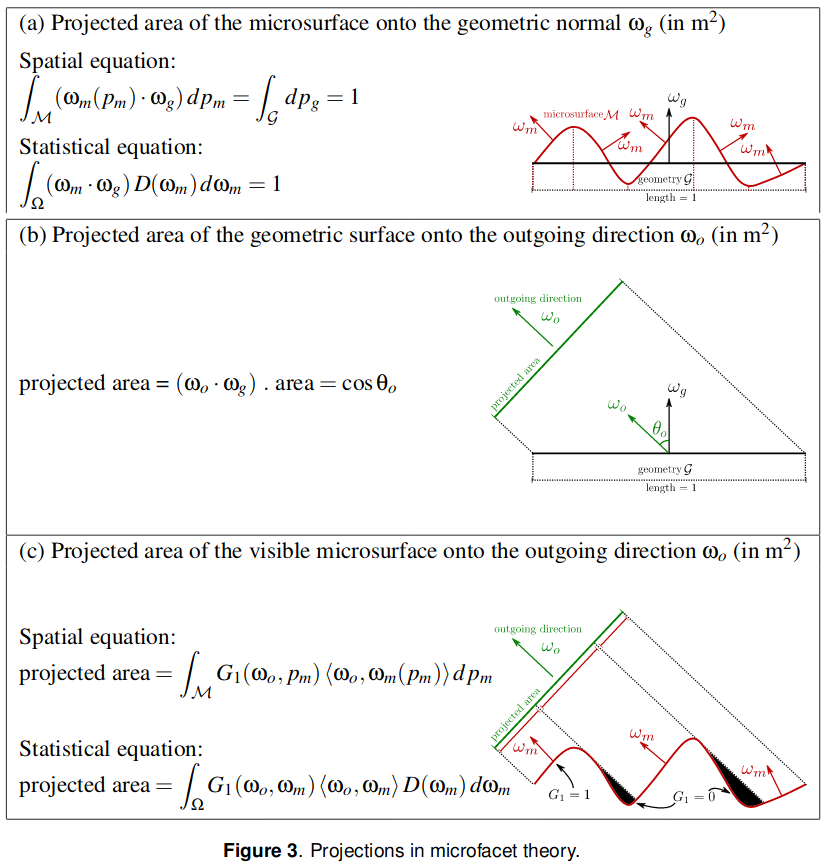
\includegraphics[width=\textwidth]{Figure3.png}
    \caption{}
    \label{fig:3}
\end{figure}

\subsection{masking関数の制約(A Constraint on the Masking Function)}

図3では、式$\eqref{eq:13}$で示される可視マイクロサーフェスの射影面積は、式$\eqref{eq:10}$で示される幾何学的表面の射影面積にピタリと一致する、というマイクロファセット理論の根本的な性質を取り上げた。この等価性は統計学的なmasking関数に以下の式で表される制約を課す。

\begin{equation}
    \boxed{
    \cos \theta_o = \int_\Omega G_1(\boldsymbol{\omega}_o, \boldsymbol{\omega}_m) \langle \boldsymbol{\omega}_o, \boldsymbol{\omega}_m \rangle D(\boldsymbol{\omega}_m) d\boldsymbol{\omega}_m
    }
    \label{eq:14}
\end{equation}

物理ベースのmasking関数$G_1$はこの制約を常に満たさなければならない。しかし、この制約は$G_1$を完全に決定するものではない。なぜなら、masking関数$G_1$は$\boldsymbol{\omega}_o$と $\boldsymbol{\omega}_m)$の2つを取る関数であり、出射方向$\boldsymbol{\omega}_o$を定めても、この制約を満たす$G_1$は無限に存在するためである。そこで、解をひとつに定めるため、第2の制約としてマイクロサーフェス・プロファイル(microsurface profile)を導入する。

これを直感的に理解する方法は、法線分布はマイクロサーフェス上の各法線の割合のみを示すヒストグラムのようなものだと考えることである。そうすると、法線分布からは法線がどのように組織しているかという情報が得られないことが分かる。そのため、マイクロサーフェスの断面図(profile)が必要になる。さらに、図\ref{fig:4}に示す通り、プロファイルの選択は、出来上がるBRDFの形状に重大な影響力を持ち得る。マイクロサーフェス・プロファイルが決まれば、masking関数は完全に決定され、その完全形式(exact form)を導き出すことができる。

\subsection{まとめ(Summary)}

"masking関数(または、幾何減衰因数(geometric attenuation factor))の中から一体どれを使えば良いの?それって物理ベースなの?"、というmasking関数に関するよくある質問がある。
この章では以下を示した。

- いずれの方向に射影しても、可視マイクロサーフェスの射影面積は幾何学的表面の射影面積と等価である。
- masking関数はこの等価性により制約を受ける。より正しく言うなら、物理ベースのmasking関数は式\eqref{eq:14}で示される数式を常に満たす。
- とはいえ、masking関数はこの制約により完全に定まるものではない。
- masking関数はマイクロサーフェス・プロファイルを選択することで一意に定まる。
- マイクロサーフェス・プロファイルはBRDFの形状に影響を及ぼす。

\begin{figure}
    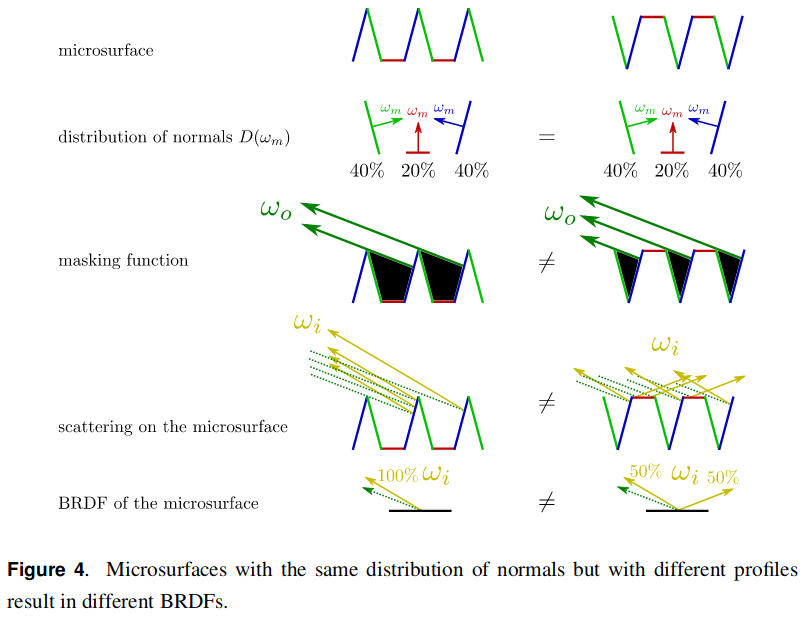
\includegraphics[width=\textwidth]{Figure4.png}
    \caption{}
    \label{fig:4}
\end{figure}

\section{マイクロファセットベースBRDF(Microfacet-Based BRDFs)}

\begin{figure}
    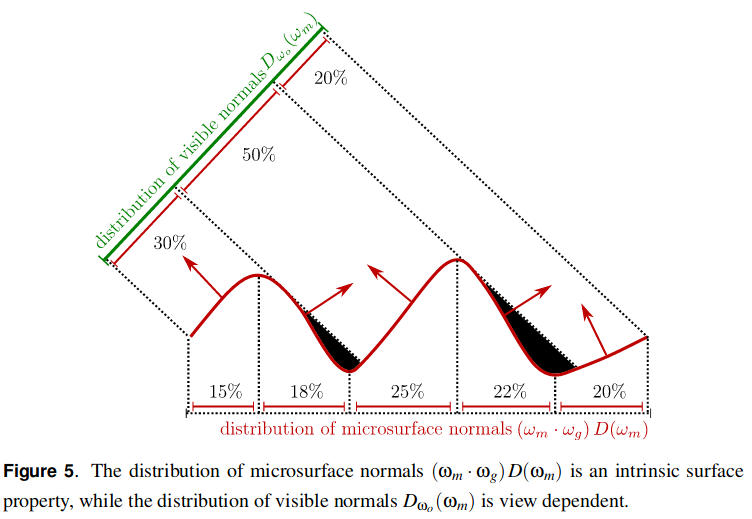
\includegraphics[width=\textwidth]{Figure5.png}
    \caption{}
    \label{fig:5}
\end{figure}

\subsection{可視法線分布(Distribution of Visible Normals)}

式\eqref{eq:1}をマイクロファセットのパラダイムで定式化すると以下のようになる。

\begin{equation}
    L(\boldsymbol{\omega}_o, \mathcal{M}) = \frac{1}{\cos\theta_o} \int_\Omega L(\boldsymbol{\omega}_o, \boldsymbol{\omega}_m) G_1(\boldsymbol{\omega}_o, \boldsymbol{\omega}_m) \langle \boldsymbol{\omega}_o, \boldsymbol{\omega}_m \rangle D(\boldsymbol{\omega}_m) d\boldsymbol{\omega}_m
    \label{eq:15}
\end{equation}

ここで、$L(\boldsymbol{\omega}_o, \mathcal{M})$はマイクロサーフェスから出射する放射輝度を、$L(\boldsymbol{\omega}_o, \boldsymbol{\omega}_m)$は法線$\boldsymbol{\omega}_m$を持つマイクロファセットから出射する放射輝度を、$\frac{1}{\cos\theta_o}$はここでは幾何学的表面の射影面積による積分を正規化する因子を表す。つまり、図\ref{fig:5}で示すように、マイクロサーフェスから出射する放射輝度は、可視法線分布(the distribution of visible normals)で重み付けされた、各マイクロファセットから出射する放射輝度の合計であると理解することができる。この可視法線分布は、各法線の射影面積とmasking関数で重み付けされた法線分布として表される。

\begin{equation}
    D_{\boldsymbol{\omega}_o}(\boldsymbol{\omega}_m) = \frac{G_1(\boldsymbol{\omega}_o, \boldsymbol{\omega}_m) \langle \boldsymbol{\omega}_o, \boldsymbol{\omega}_m \rangle D(\boldsymbol{\omega}_m)}{cos\theta_o}
    \label{eq:16}
\end{equation}

この可視法線分布$D_{\boldsymbol{\omega}_o}(\boldsymbol{\omega}_m)$は正規化されているということが重要で、この性質を利用すれば、放射輝度の平均を取るための重み関数として用いることができる。

\begin{equation}
    L(\boldsymbol{\omega}_o, \mathcal{M}) = \int_\Omega L(\boldsymbol{\omega}_o, \boldsymbol{\omega}_m) D_{\boldsymbol{\omega}_o}(\boldsymbol{\omega}_m) d\boldsymbol{\omega}_m
    \label{eq:17}
\end{equation}

\ref{sec:2.1}や図\ref{fig:1}で示した通り、放射輝度の平均はその重み関数が正規化されている場合にのみ有効である。上の式は、正しく正規化されることが保証されている式\eqref{eq:1}の分母の積分をmasking関数$G_1$で表したものであるため、うまく定義されている(well defined)と言える。もちろん、式\eqref{eq:14}を用いて、式\eqref{eq:16}を$\cos\theta_o$に入れ替えることで、この法線分布が正規化されていることを確かめることができる。

\begin{equation}
    \begin{split}
        \int_\Omega D_{\boldsymbol{\omega}_o}(\boldsymbol{\omega}_m) d\boldsymbol{\omega}_m
        &= \int_\Omega \frac{G_1(\boldsymbol{\omega}_o, \boldsymbol{\omega}_m) \langle \boldsymbol{\omega}_o, \boldsymbol{\omega}_m \rangle D(\boldsymbol{\omega}_m)}{\cos\theta_o} d\boldsymbol{\omega}_m \\
        &= \frac{\int_\Omega G_1(\boldsymbol{\omega}_o, \boldsymbol{\omega}_m) \langle \boldsymbol{\omega}_o, \boldsymbol{\omega}_m \rangle D(\boldsymbol{\omega}_m) d\boldsymbol{\omega}_m}{\int_\Omega G_1(\boldsymbol{\omega}_o, \boldsymbol{\omega}_m) \langle \boldsymbol{\omega}_o, \boldsymbol{\omega}_m \rangle D(\boldsymbol{\omega}_m)d \boldsymbol{\omega}_m} \\
        &= 1
    \end{split}
    \label{eq:18}
\end{equation}

同様にして、式\eqref{eq:15}と式\eqref{eq:17}から平均出射照射輝度(average outgoing radiance)が正しく正規化されていることを強調する式\eqref{eq:1}と同じ形式で表現できる。

\begin{equation}
    L(\boldsymbol{\omega}_o, \mathcal{M}) = \frac{\int_\Omega L(\boldsymbol{\omega}_o, \boldsymbol{\omega}_m) G_1(\boldsymbol{\omega}_o, \boldsymbol{\omega}_m) \langle \boldsymbol{\omega}_o, \boldsymbol{\omega}_m \rangle D(\boldsymbol{\omega}_m) d \boldsymbol{\omega}_m}{\int_\Omega G_1(\boldsymbol{\omega}_o, \boldsymbol{\omega}_m) \langle \boldsymbol{\omega}_o, \boldsymbol{\omega}_m \rangle D(\boldsymbol{\omega}_m)d \boldsymbol{\omega}_m}
    \label{eq:19}
\end{equation}

\subsection{BRDFの構築(Construction of the BRDF)}
\label{sec:3.2}

可視法線分布をもとにBRDFを作成することを考える。各マイクロファセットの放射輝度$L(\boldsymbol{\omega}_o, \boldsymbol{\omega}_m)$は、各マクロファセットと関連したマイクロBRDF(micro-BRDF)の項$\rho_{\mathcal M}(\boldsymbol{\omega}_o, \boldsymbol{\omega}_i, \boldsymbol{\omega}_m)$を入射する放射輝度$L(\boldsymbol{\omega}_i)$とともに入射方向の領域$\Omega_i$上で積分したものとして表される。

\begin{equation}
    L(\boldsymbol{\omega}_o, \boldsymbol{\omega}_m) = \int_{\Omega_i} \frac{dL(\boldsymbol{\omega}_o, \boldsymbol{\omega}_m)}{d\boldsymbol{\omega}_i} d\boldsymbol{\omega}_i = \int_{\Omega_i} \rho_{\mathcal M}(\boldsymbol{\omega}_o, \boldsymbol{\omega}_i, \boldsymbol{\omega}_m) \langle \boldsymbol{\omega}_i, \boldsymbol{\omega}_m \rangle L(\boldsymbol{\omega}_i) d\boldsymbol{\omega}_i
    \label{eq:20}
\end{equation}

ここで、マイクロBRDF$\rho_{\mathcal M}(\boldsymbol{\omega}_o, \boldsymbol{\omega}_i, \boldsymbol{\omega}_m)$は出射する放射輝度の微分$dL(\boldsymbol{\omega}_o, \boldsymbol{\omega}_m)$と入射する放射照度の微分$\langle \boldsymbol{\omega}_i, \boldsymbol{\omega}_m \rangle L(\boldsymbol{\omega}_i) d\boldsymbol{\omega}_i$の割合を表す。

\begin{equation}
    \rho_{\mathcal M}(\boldsymbol{\omega}_o, \boldsymbol{\omega}_i, \boldsymbol{\omega}_m) = \frac{dL(\boldsymbol{\omega}_o, \boldsymbol{\omega}_m)}{\langle \boldsymbol{\omega}_i, \boldsymbol{\omega}_m \rangle L(\boldsymbol{\omega}_i) d\boldsymbol{\omega}_i}
    \label{eq:21}
\end{equation}

次に、式\eqref{eq:17}を入射する放射照度に関して微分し、式\eqref{eq:21}により$dL(\boldsymbol{\omega}_o, \boldsymbol{\omega}_m)$を置き換える。

\begin{equation}
    \begin{split}
        dL(\boldsymbol{\omega}_o, \mathcal{M})
        &= \int_{\Omega} dL(\boldsymbol{\omega}_o, \boldsymbol{\omega}_m) D_{\boldsymbol{\omega}_o}(\boldsymbol{\omega}_m) d\boldsymbol{\omega}_m \\
        &= L(\boldsymbol{\omega}_i) d\boldsymbol{\omega}_i \int_{\Omega} \rho_{\mathcal M}(\boldsymbol{\omega}_o, \boldsymbol{\omega}_i, \boldsymbol{\omega}_m) \langle \boldsymbol{\omega}_i, \boldsymbol{\omega}_m \rangle D_{\boldsymbol{\omega}_o}(\boldsymbol{\omega}_m) d\boldsymbol{\omega}_m
    \end{split}
    \label{eq:22}
\end{equation}

ここで、$L(\boldsymbol{\omega}_i)d\boldsymbol{\omega}_i$は$\boldsymbol{\omega}_m$に依存していないので積分の外に出すことができる。
マクロBRDF(macro-BRDF)は以下の式で定義されるため、

\begin{equation}
    dL(\boldsymbol{\omega}_o, \mathcal{M}) = \rho(\boldsymbol{\omega}_o, \boldsymbol{\omega}_i) \cos\theta_i L(\boldsymbol{\omega}_i) d\boldsymbol{\omega}_i
    \label{eq:23}
\end{equation}

以下が成り立つ。

\begin{equation}
    \begin{split}
        \rho(\boldsymbol{\omega}_o, \boldsymbol{\omega}_i)
        &= \frac{dL(\boldsymbol{\omega}_o, \mathcal M)}{\cos\theta_i L(\boldsymbol{\omega}_i) d\boldsymbol{\omega}_i} \\
        &= \frac{1}{\cos\theta_i} \int_{\Omega} \rho_{\mathcal M}(\boldsymbol{\omega}_o, \boldsymbol{\omega}_i, \boldsymbol{\omega}_m) \langle \boldsymbol{\omega}_i, \boldsymbol{\omega}_m \rangle D_{\boldsymbol{\omega}_o}(\boldsymbol{\omega}_m) d\boldsymbol{\omega}_m
    \end{split}
    \label{eq:24}
\end{equation}

$D_{\boldsymbol{\omega}_o}(\boldsymbol{\omega}_m)$を式\eqref{eq:16}で置き換えれば、以下が成り立つ。

\begin{equation}
    \begin{split}
        \rho(\boldsymbol{\omega}_o, \boldsymbol{\omega}_i)
        &= \frac{1}{\cos\theta_o \cos\theta_i} \int_{\Omega} \rho_{\mathcal M}(\boldsymbol{\omega}_o, \boldsymbol{\omega}_i, \boldsymbol{\omega}_m) \langle \boldsymbol{\omega}_o, \boldsymbol{\omega}_m \rangle \langle \boldsymbol{\omega}_i, \boldsymbol{\omega}_m \rangle G_1(\boldsymbol{\omega}_o, \boldsymbol{\omega}_m) D(\boldsymbol{\omega}_m) d\boldsymbol{\omega}_m \\
        &= \frac{1}{|\boldsymbol{\omega}_g \cdot \boldsymbol{\omega}_o| |\boldsymbol{\omega}_g \cdot \boldsymbol{\omega}_i|} \int_{\Omega} \rho_{\mathcal M}(\boldsymbol{\omega}_o, \boldsymbol{\omega}_i, \boldsymbol{\omega}_m) \langle \boldsymbol{\omega}_o, \boldsymbol{\omega}_m \rangle \langle \boldsymbol{\omega}_i, \boldsymbol{\omega}_m \rangle G_1(\boldsymbol{\omega}_o, \boldsymbol{\omega}_m) D(\boldsymbol{\omega}_m) d\boldsymbol{\omega}_m
    \end{split}
    \label{eq:25}
\end{equation}

この式は1回目のバウンス(bounce)の後、表面付近(vicinity of the surface)を離れる\textbf{前}に、どれだけのレイ(ray)が反射されたかについてモデル化するだけである(図\ref{fig:6}(b))、という理解が重要である。一方で、BRDFモデルは、すべてのmicroscattering(微正面での散乱)を経て、表面を離れた\textbf{後}にレイがどのように分布しているかを説明しなければならない。反射したレイが表面付近を離れる前に再びマイクロサーフェスに当たって別の方向に反射することもあり得るため、表面付近を離れるのが前か後かによってこの分布は異なってくる(図\ref{fig:6}(d))。ここで導出されるBRDFモデルは、表面での1回目のバウンスのみを説明し、複数回のバウンスに関与するレイ(図\ref{fig:6}(c)の黒矢印)はモデルからは排除される。これは、shadowing関数を導入することで達成される。実際には、masking関数$G_1$をmasking-shadowing関数$G_2$に置き換える。

\begin{equation}
    \rho(\boldsymbol{\omega}_o, \boldsymbol{\omega}_i) = \frac{1}{|\boldsymbol{\omega}_g \cdot \boldsymbol{\omega}_o| |\boldsymbol{\omega}_g \cdot \boldsymbol{\omega}_i|} \int_{\Omega} \rho_{\mathcal M}(\boldsymbol{\omega}_o, \boldsymbol{\omega}_i, \boldsymbol{\omega}_m) \langle \boldsymbol{\omega}_o, \boldsymbol{\omega}_m \rangle \langle \boldsymbol{\omega}_i, \boldsymbol{\omega}_m \rangle G_2(\boldsymbol{\omega}_o, \boldsymbol{\omega}_i, \boldsymbol{\omega}_m) D(\boldsymbol{\omega}_m) d\boldsymbol{\omega}_m
    \label{eq:26}
\end{equation}

\subsection{鏡面的マイクロファセットにおけるBRDFの構築(Construction of the BRDF with specular microfacets)}

鏡のようなマイクロファセットのマイクロBRDFは以下のようになる。

\begin{equation}
    \begin{split}
        \rho_{\mathcal M}(\boldsymbol{\omega}_o, \boldsymbol{\omega}_i, \boldsymbol{\omega}_m)
        &= \left\lVert \frac{\partial \boldsymbol{\omega}_h}{\partial \boldsymbol{\omega}_i} \right\rVert \frac{F(\boldsymbol{\omega}_o, \boldsymbol{\omega}_h) \delta_{\boldsymbol{\omega}_h}(\boldsymbol{\omega}_m)}{| \boldsymbol{\omega}_i \cdot \boldsymbol{\omega}_h |} \\
        &= \frac{F(\boldsymbol{\omega}_o, \boldsymbol{\omega}_h) \delta_{\boldsymbol{\omega}_h}(\boldsymbol{\omega}_m)}{4 | \boldsymbol{\omega}_i \cdot \boldsymbol{\omega}_h |^2}
    \end{split}
    \label{eq:27}
\end{equation}

ここで、$\left\lVert \frac{\partial \boldsymbol{\omega}_h}{\partial \boldsymbol{\omega}_i} \right\rVert = \frac{1}{4|\boldsymbol{\omega}_i \cdot \boldsymbol{\omega}_h|}$は鏡映変換(reflection transformation)のヤコビアン(Jacobian)を、$F$はフレネル項を表す。式\eqref{eq:26}について、$\rho_{\mathcal M}(\boldsymbol{\omega}_o, \boldsymbol{\omega}_i, \boldsymbol{\omega}_m)$をを式\eqref{eq:27}で、$D_{\boldsymbol{\omega}_o}(\boldsymbol{\omega}_m)$を式\eqref{eq:16}で置き換えると、以下が求められる。

\begin{equation}
    \rho(\boldsymbol{\omega}_o, \boldsymbol{\omega}_i) = \frac{1}{|\boldsymbol{\omega}_g \cdot \boldsymbol{\omega}_o| |\boldsymbol{\omega}_g \cdot \boldsymbol{\omega}_i|} \int_{\Omega} \frac{F(\boldsymbol{\omega}_o, \boldsymbol{\omega}_h)\delta_{\boldsymbol{\omega}_h}(\boldsymbol{\omega}_m)}{4|\boldsymbol{\omega}_i \cdot \boldsymbol{\omega}_h|^2} \langle \boldsymbol{\omega}_o, \boldsymbol{\omega}_m \rangle \langle \boldsymbol{\omega}_i, \boldsymbol{\omega}_m \rangle G_2(\boldsymbol{\omega}_o, \boldsymbol{\omega}_i, \boldsymbol{\omega}_m) D(\boldsymbol{\omega}_m) d\boldsymbol{\omega}_m
    \label{eq:28}
\end{equation}

デルタ関数$\delta_{\boldsymbol{\omega}_h}(\boldsymbol{\omega}_m)$の積分は$\boldsymbol{\omega}_m = \boldsymbol{\omega}_h$とした被積分関数に置き換えることができ、$\boldsymbol{\omega}_o \cdot \boldsymbol{\omega}_h = \boldsymbol{\omega}_i \cdot \boldsymbol{\omega}_h$が成り立つため、式を以下にまで簡略化できる。

\begin{equation}
    \rho(\boldsymbol{\omega}_o, \boldsymbol{\omega}_i) = \frac{F(\boldsymbol{\omega}_o, \boldsymbol{\omega}_h) G_2(\boldsymbol{\omega}_o, \boldsymbol{\omega}_i, \boldsymbol{\omega}_h) D(\boldsymbol{\omega}_h)}{4|\boldsymbol{\omega}_g \cdot \boldsymbol{\omega}_o| |\boldsymbol{\omega}_g \cdot \boldsymbol{\omega}_i|}
    \label{eq:29}
\end{equation}

これにより、よく知られた、鏡面的マイクロファセットベースBRDFの数式を求めることができる。

\subsection{拡散的マイクロファセットにおけるBRDFの構築(Construction of the BRDF with diffuse microfacets)}

拡散的マイクロファセットのマイクロBRDFは定数である。

\begin{equation}
    \rho_{\mathcal M}(\boldsymbol{\omega}_o, \boldsymbol{\omega}_i, \boldsymbol{\omega}_m) = \frac{1}{\pi}
    \label{eq:30}
\end{equation}

式\eqref{eq:26}について、$\rho_{\mathcal M}(\boldsymbol{\omega}_o, \boldsymbol{\omega}_i, \boldsymbol{\omega}_m)$をを式\eqref{eq:30}で、$D_{\boldsymbol{\omega}_o}(\boldsymbol{\omega}_m)$を式\eqref{eq:16}で置き換えると、以下が求められる。

\begin{equation}
    \rho(\boldsymbol{\omega}_o, \boldsymbol{\omega}_i) = \frac{1}{\pi} \frac{1}{|\boldsymbol{\omega}_g \cdot \boldsymbol{\omega}_o| |\boldsymbol{\omega}_g \cdot \boldsymbol{\omega}_i|} \int_{\Omega} \langle \boldsymbol{\omega}_o, \boldsymbol{\omega}_m \rangle \langle \boldsymbol{\omega}_i, \boldsymbol{\omega}_m \rangle G_2(\boldsymbol{\omega}_o, \boldsymbol{\omega}_i, \boldsymbol{\omega}_m) D(\boldsymbol{\omega}_m) d\boldsymbol{\omega}_m
    \label{eq:31}
\end{equation}

この式は解析的な解(analytical solution)ではない。OrenとNayarは、$D$が --- 紛らわしいがBeckmann分布ではなく --- 球面ガウス関数(spherical Gaussian)であり、$G_2$がV型空洞(V-cavity)のmasking-shadowing関数である場合の、この関数の解析的フィッティングを提案している。

\subsection{BRDFの正規化テスト(The BRDF Normalization Test)}

\paragraph{White Furnaceテスト(The White Furnace Test)}

双方向散乱分布関数(BSDF)$s$は、上半分の半球上に定義される双方向反射率分布関数(BRDF)$\rho$と、下半分の半球上に定義される双方向透過率分布関数(BTDF)$t$の和である。

\begin{equation}
    s(\boldsymbol{\omega}_o, \boldsymbol{\omega}_i) = \rho(\boldsymbol{\omega}_o, \boldsymbol{\omega}_i) + t(\boldsymbol{\omega}_o, \boldsymbol{\omega}_i)
    \label{eq:32}
\end{equation}

入射する放射輝度が吸収されない表面である場合、レイの放射輝度は散乱中において完全に保存される。したがって、表面での吸収が$0$のときに散乱したレイの分布が完全に正規化されるかどうかは、マイクロファセットベースの散乱モデルで確認しておきたい重要な性質のひとつである。

\begin{equation}
    \int_{\Omega_i} s(\boldsymbol{\omega}_o, \boldsymbol{\omega}_i) |\boldsymbol{\omega}_g \cdot \boldsymbol{\omega}_i| d\boldsymbol{\omega}_i = 1 \forall \boldsymbol{\omega}_o
    \label{eq:33}
\end{equation}

フレネル項が常に$1$であるなら、レイは透過が一切起こらないため、BTDFは$t = 0$となり、散乱モデルは完全にBRDFによって定義される(つまり、$s = \rho$となる)。この場合、レイはエネルギーを失うことなくすべからく反射され、その分布は正規化される。これはWhite Furnaceテストの式として以下のようにモデル化される。

\begin{equation}
    \int_{\Omega_i} \rho(\boldsymbol{\omega}_o, \boldsymbol{\omega}_i) |\boldsymbol{\omega}_g \cdot \boldsymbol{\omega}_i| d\boldsymbol{\omega}_i = 1
    \label{eq:34}
\end{equation}

直観として、これは、出射方向から放たれた(cast)レイが何度か散乱してから表面を離れる様を表現していると考えることができる。しかし、図\ref{fig:6}(c)や\ref{sec:3.2}が示す通り、複数回バウンスするレイはshadowing関数によりBRDFから取り除かれているため、一般的な解析的BRDFはマイクロサーフェス上での複数回の散乱をモデル化していない。"完璧な反射板(perfect reflector)"としてのマイクロサーフェスをパラメータ化したものであっても、一般的なBRDFモデルでは積分が$1$にならず、White Furnaceテスト式を満たさないのは、ここに理由がある。

\paragraph{Weak White Furnaceテスト(The Weak White Furnace Test)}

White Furnaceテストは、最初の散乱事象しか組み込まれていない、一般的なBRDFモデルを検証するのには使えない。しかしながら、一般的なBRDFモデルが満たすべき、制限を緩和したテストを設計することはできる。1回目のバウンスの直後に表面を離れる\textbf{前}であるレイの分布が正規化されていることを確かめればよいのだ(図\ref{fig:6}(b))。これは、masking-shadowing関数をmaskingのみに置き換える($G_2(\boldsymbol{\omega}_o, \boldsymbol{\omega}_i, \boldsymbol{\omega}_h) = G_1(\boldsymbol{\omega}_o, \boldsymbol{\omega}_h)$)ことで達成できる。式\eqref{eq:29}からフレネル項とshadowing関数を除けば以下の式が求められる。

\begin{equation}
    \rho(\boldsymbol{\omega}_o, \boldsymbol{\omega}_i) = \frac{G_1(\boldsymbol{\omega}_o, \boldsymbol{\omega}_h) D(\boldsymbol{\omega}_h)}{4|\boldsymbol{\omega}_g \cdot \boldsymbol{\omega}_o| |\boldsymbol{\omega}_g \cdot \boldsymbol{\omega}_i|}
    \label{eq:35}
\end{equation}

この式でWhite Furnaceテストを置き換えれば、Weak White Furnaceテストの式が以下のように求められる。

\begin{equation}
    \boxed{
    \int_{\Omega_i} \frac{G_1(\boldsymbol{\omega}_o, \boldsymbol{\omega}_h) D(\boldsymbol{\omega}_h)}{4|\boldsymbol{\omega}_g \cdot \boldsymbol{\omega}_o|} d\boldsymbol{\omega}_i = 1
    }
    \label{eq:36}
\end{equation}

この条件は、式\eqref{eq:14}を満足する適切なmasking関数$G_1$によってのみ満たすことができる。

式\eqref{eq:31}を$G_2(\boldsymbol{\omega}_o, \boldsymbol{\omega}_i, \boldsymbol{\omega}_h) = G_1(\boldsymbol{\omega}_o, \boldsymbol{\omega}_h)$で置き換え、入射方向に対して積分することにより、拡散的マイクロファセットにおけるBRDFのための同様のテストを定義した。

\begin{equation}
    \begin{split}
        & \int_{\Omega_i} \frac{1}{\pi} \frac{1}{|\boldsymbol{\omega}_g \cdot \boldsymbol{\omega}_o| |\boldsymbol{\omega}_g \cdot \boldsymbol{\omega}_i|} \int_{\Omega} \langle \boldsymbol{\omega}_o, \boldsymbol{\omega}_m \rangle \langle \boldsymbol{\omega}_i, \boldsymbol{\omega}_m \rangle G_1(\boldsymbol{\omega}_o, \boldsymbol{\omega}_m) D(\boldsymbol{\omega}_m) d\boldsymbol{\omega}_m |\boldsymbol{\omega}_g \cdot \boldsymbol{\omega}_i| d\boldsymbol{\omega}_i \\
        &= \frac{1}{\pi} \frac{1}{|\boldsymbol{\omega}_g \cdot \boldsymbol{\omega}_o|} \int_{\Omega_i} \int_{\Omega} \langle \boldsymbol{\omega}_o, \boldsymbol{\omega}_m \rangle \langle \boldsymbol{\omega}_i, \boldsymbol{\omega}_m \rangle G_1(\boldsymbol{\omega}_o, \boldsymbol{\omega}_m) D(\boldsymbol{\omega}_m) d\boldsymbol{\omega}_m d\boldsymbol{\omega}_i \\
        &= 1
    \end{split}
    \label{eq:37}
\end{equation}

\begin{figure}
    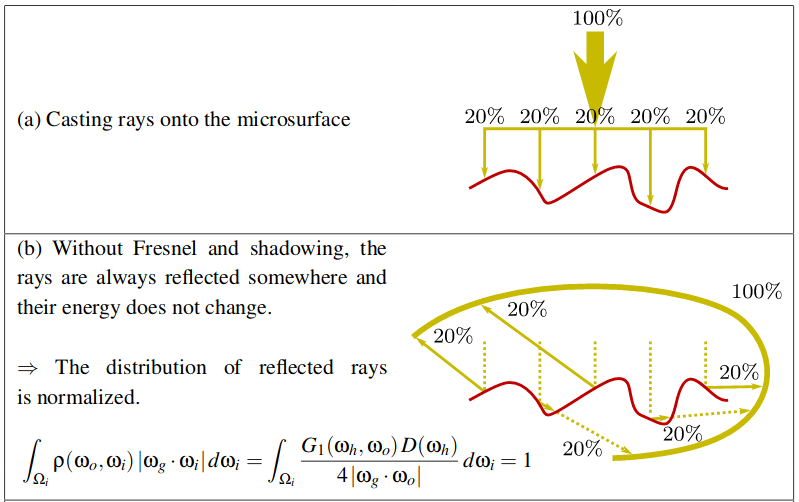
\includegraphics[width=\textwidth]{Figure6_1.png}
    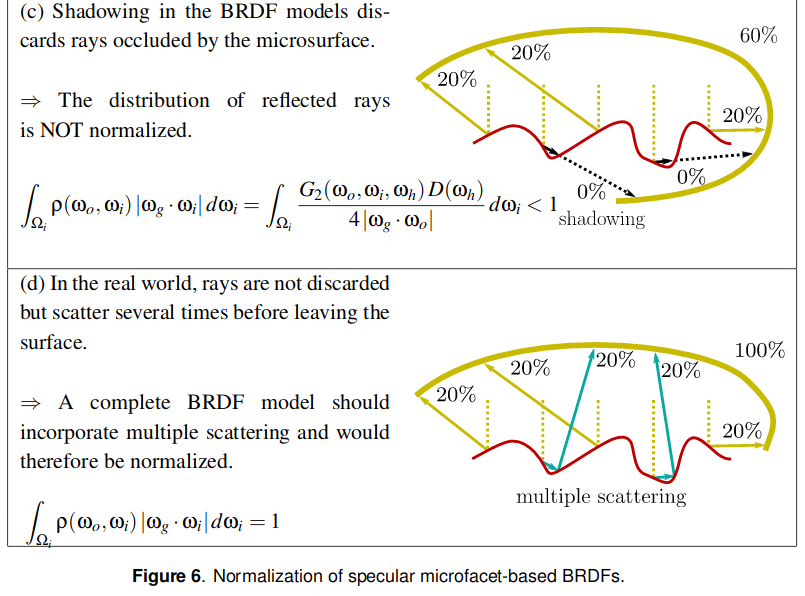
\includegraphics[width=\textwidth]{Figure6_2.png}
    \caption{}
    \label{fig:6}
\end{figure}

\subsection{まとめ(Summary)}

BRDFの正規化に関するよくある質問として、"マイクロファセットベースBRDFが積分しても$1$にならないんだけど、これってちゃんと正規化されてないんじゃないの?"というものがある。

このセクションでは、以下のアイデアを開発することで、この質問に対する答えとした。

\begin{itemize}
\item BRDFは可視法線分布により生成される。
\item 可視法線分布は、BRDFがエネルギーを保存することを保証するために正規化されていなければならない。
\item 可視法線分布の正規化係数はmasking関数である。
\item マイクロファセットベースBRDFは正規化されるべきである。すなわち、吸収せず、透過しない材質ではピッタリ1に積分される。
\item マイクロファセットベースBRDFのshadowing関数はマイクロサーフェスにおける複数回の散乱事象から最初の散乱事象を切り離すために用いる。shadowingは2回以上の散乱事象を破棄(0に設定)し、複数回の散乱事象をモデル化する項が存在しない場合にはBRDFを人為的に非正規化されたままにする。
\item マイクロファセットベースBRDFの標準形は、フレネルとshadowingを取り除いて、masking関数によって正規化される。物理ベースmasking関数は常に式\eqref{eq:36}と\eqref{eq:37}を満たす。これは我々が"Weak White Furnaceテスト"と呼ぶものである。
\end{itemize}

shadowingが組み込まれていないWeak White Furnaceテストは、masking関数が物理的に正しいことを確認する簡単な方法である。これは、一般的なBRDFモデルがshadowingを取り除いて用いられるべきであるという意味ではないことに特に気をつけたい。shadowingとは、一般的なBRDFモデルには組み込まれていない複数回のバウンスの後に反射するエネルギーから最初のバウンスの後に反射するエネルギーを分離することである。

\section{一般的な物理ベースmasking関数と非物理ベースmasking関数(Common Physically Based and Non-Physically Based Masking Functions)}

\subsection{Smithのマイクロサーフェス・プロファイル(The Smith Microsurface Profile)}
\label{sec:4.1}

\paragraph{法線/masking独立(Normal/Masking Independence)}

Smithのマイクロサーフェス・プロファイルは、マイクロサーフェスが自己相関して(autocorrelate)いない、すなわち、マイクロサーフェスの一点での高さ(または法線)と、(最近接点であっても)どの近傍点の高さとの間にも相関(correlation)がないことを仮定する。これは、図\ref{fig:7}の右側が示す通り、連続的な表面ではなくランダムなマイクロファセットの集合であることを意味する。つまり、マイクロサーフェスの高さや法線は独立した乱数である。

\begin{figure}
    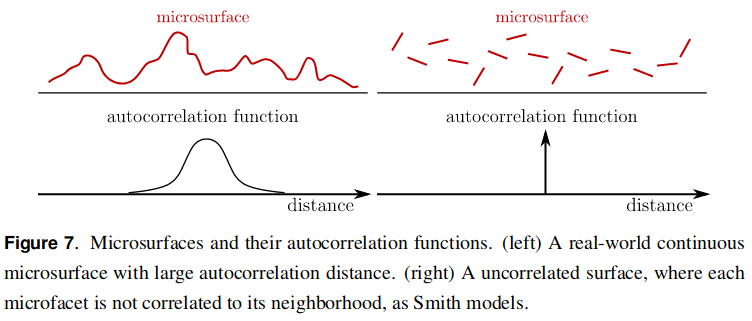
\includegraphics[width=\textwidth]{Figure7.png}
    \caption{}
    \label{fig:7}
\end{figure}

このモデルから、masking関数によって与えられる確率$G_1(\boldsymbol{\omega}_o, \boldsymbol{\omega}_m)$は、背面を向いていない($\boldsymbol{\omega}_o \cdot \boldsymbol{\omega}_m > 0$)法線について、法線の向き$\boldsymbol{\omega}_m$に対して独立である、ということを導き出せる。法線$\boldsymbol{\omega}_m$はマイクロファセットの\textbf{近い(local)}所での性質である一方、maskingの原因となる潜在的な遮蔽(potential occlusion responsible for masking)はマイクロサーフェス上の他の場所で起こる、すなわち、マイクロファセットの\textbf{遠い(distant)}所での性質であることが、直観として理解できる。ただし、依然としてミクロスケールでの話である。マイクロサーフェスが自己相関しないため、近い所での性質は遠い所での性質に対して独立であり、masking関数は以下の分割された形式で表現できる。

\begin{equation}
    G_1(\boldsymbol{\omega}_o, \boldsymbol{\omega}_m) = G_1^{\text{local}}(\boldsymbol{\omega}_o, \boldsymbol{\omega}_m) G_1^{\text{dist}}(\boldsymbol{\omega}_o)
    \label{eq:38}
\end{equation}

ここで、近い所でのmasking関数は、背面のマイクロファセットを破棄するかどうかを二値化したものである。

\begin{equation}
    G_1^{\text{local}}(\boldsymbol{\omega}_o, \boldsymbol{\omega}_m) = \chi^+(\boldsymbol{\omega}_o \cdot \boldsymbol{\omega}_m)
    \label{eq:39}
\end{equation}

そして、遠い所でのmasking関数$G_1^{\text{dist}}(\boldsymbol{\omega}_o)$は、localな向き$\boldsymbol{\omega}_m$に対して独立である、マイクロサーフェスの遠くの点による遮蔽確率を表す。

\paragraph{masking関数の導出(Derivation of the Masking Function)}

式\eqref{eq:38}で式\eqref{eq:14}のmasking関数を展開することで、以下の式が求められる。

\begin{equation}
    \begin{split}
        \cos\theta_o
        &= \int_{\Omega} G_1(\boldsymbol{\omega}_o, \boldsymbol{\omega}_m) \langle \boldsymbol{\omega}_o, \boldsymbol{\omega}_m \rangle D(\boldsymbol{\omega}_m) d\boldsymbol{\omega}_m \\
        &= \int_{\Omega} G_1^{\text{local}}(\boldsymbol{\omega}_o, \boldsymbol{\omega}_m) G_1^{\text{dist}}(\boldsymbol{\omega}_o) \langle \boldsymbol{\omega}_o, \boldsymbol{\omega}_m \rangle D(\boldsymbol{\omega}_m) d\boldsymbol{\omega}_m \\
        &= \int_{\Omega} \chi^+(\boldsymbol{\omega}_o \cdot \boldsymbol{\omega}_m) G_1^{\text{dist}}(\boldsymbol{\omega}_o) \langle \boldsymbol{\omega}_o, \boldsymbol{\omega}_m \rangle D(\boldsymbol{\omega}_m) d\boldsymbol{\omega}_m \\
        &=  G_1^{\text{dist}}(\boldsymbol{\omega}_o) \int_{\Omega} \langle \boldsymbol{\omega}_o, \boldsymbol{\omega}_m \rangle D(\boldsymbol{\omega}_m) d\boldsymbol{\omega}_m
    \end{split}
    \label{eq:40}
\end{equation}

ここで、$G_1^{\text{dist}}(\boldsymbol{\omega}_o)$は$\boldsymbol{\omega}_m$に依存しないため積分の外に出すことができる。また、$\boldsymbol{\omega}_o \cdot \boldsymbol{\omega}_m < 0$のとき$0$になるクランプされた内積がすでにあるので、階段関数$\chi^+(\boldsymbol{\omega}_o \cdot \boldsymbol{\omega}_m)$は冗長になるため取り除かれる。よって、出射方向$\boldsymbol{\omega}_o$から見て背面でない法線のmasking関数は以下の式で表される。

\begin{equation}
    G_1^{\text{dist}}(\boldsymbol{\omega}_o) = \frac{\cos\theta_o}{\int_{\Omega} \langle \boldsymbol{\omega}_o, \boldsymbol{\omega}_m \rangle D(\boldsymbol{\omega}_m) d\boldsymbol{\omega}_m}
    \label{eq:41}
\end{equation}

したがって、完全なmasking関数は以下の式で表される。

\begin{equation}
    \boxed{
    G_1(\boldsymbol{\omega}_o, \boldsymbol{\omega}_m) = \chi^+(\boldsymbol{\omega}_o \cdot \boldsymbol{\omega}_m) \frac{\cos\theta_o}{\int_{\Omega} \langle \boldsymbol{\omega}_o, \boldsymbol{\omega}_m \rangle D(\boldsymbol{\omega}_m) d\boldsymbol{\omega}_m}
    }
    \label{eq:42}
\end{equation}

これはAshikhminらによる法線/masking独立における厳密な(exact)masking関数の積分形式である。彼らはこの積分式をmasking関数の前計算に用いた。その計算結果は実行時に効率的な評価を行うためのテーブルに格納していた。

\paragraph{Smithのmasking関数(The Smith Masking Function)}

この文献では、Smithのmasking関数は$\frac{1}{1 + \Lambda(\boldsymbol{\omega}_o)}$の形で表される。この関数はマイクロサーフェスの傾斜(slopes)における積分を表し、この形式はmasking確率をレイトレーシングによって定式化(formulation)することにより導かれる。この定式化の欠点(drawback)は結果の厳密さに重点が置かれていないことにある。このことで、Smithのmasking関数はたびたび近似として扱われている。

Ashikhminらの導出が同じ結果につながり、厳密さに重点が置かれているという利点を持つことを示した。つまり、積分範囲を法線から傾斜空間に変更することで、--- \ref{sec:A}で導き出されるように、 --- 式\eqref{eq:41}は以下の式で表すことができる。

\begin{equation*}
    G_1^{\text{dist}}(\boldsymbol{\omega}_o, \boldsymbol{\omega}_m) = \frac{1}{1 + \Lambda(\boldsymbol{\omega}_o)}
\end{equation*}

そして、式\eqref{eq:42}を以下の式に書き直すことができる。

\begin{equation}
    \boxed{
    G_1(\boldsymbol{\omega}_o, \boldsymbol{\omega}_m) = \frac{\chi^+(\boldsymbol{\omega}_o \cdot \boldsymbol{\omega}_m)}{1 + \Lambda(\boldsymbol{\omega}_o)}
    }
    \label{eq:43}
\end{equation}

ここで、$\frac{1}{1 + \Lambda(\boldsymbol{\omega}_o)}$はSmithのmasking関数の一般的な形式であり、様々な確率論的表面に対する閉形式の解法(closed-form solutions)が利用できる。したがって、法線/masking独立の仮定の下では、Smithのmasking関数は厳密である。

\paragraph{性質(Properties)}

いまだに、解析的関数を計測データと比較するとしたら、モデルの予測は正確だが厳密ではないことが分かるだろう。もちろん、Smithは彼の定式を現実の測定値を比較し、それが良く適合しているが、それでもなお近似であることを発見している。しかし、彼の定式は彼のフレームワークの中でならば厳密であるため、その近似は彼の導出に起因してない。統計学的モデル(例えば、Gaussian statistics)で現実の表面を説明しようとすることや、法線/masking独立を仮定することに起因している。

Smithのモデルにより仮定される相関のないマイクロサーフェスは、いくつかのメタリックなカーペイントに見られる、"金属フレーク(metal flakes)"想起させる(reminiscent)。しかし、現実での連続的な表面はより広い相関のある関数を持つ。BourlierらはSmithのmasking関数を、異なる自己相関関数(GaussianとLorentzian)を持つランダムな荒い面を数値的に計測したmasking関数を比較した。彼らの調査の結果は、ランダムな表面上の相関を無視する(neglect)ことで生まれる誤差(error)は、観測角が$\tan(\theta) / \alpha > 0.5$のときのみに顕著である(noticeable)、としている。ここで、$\sigma^2 = \frac{\alpha^2}{2}$は傾斜の分散である。Smithのmasking関数はこの場合に若干の過大な推定(overestimations)が発生する傾向がある。Smithのmasking関数が一般的に相関のある表面上でも正確であり、相関があるmasking関数に対する解析的な解が存在しないことを考えれば、コンピュータグラフィクスの文脈においてSmithのmasking関数を適用することは合理的(reasonable)であるように見える。しかしながら、Ashikhminらによって指摘されている通り、繰り返すパターンや構造的なパターン(例えば、織物(fabric))における非ランダムな表面上の相関の影響は、重要性が高くなる可能性があり、専用のモデルに組み込まれなければならない。

\paragraph{Smithの平均化されたmasking関数(The Smith Averaged Masking Functions)}

Smithは、高さや法線のような、マイクロサーフェスの異なる量を平均化したmasking関数導き出した。式\eqref{eq:43}で表されるmasking関数$G_1(\boldsymbol{\omega}_o, \boldsymbol{\omega}_m)$はマイクロサーフェスの高さを平均化した形式であり、BRDFの中で使われなければならないものである。もちろん、高さはBRDFに関係する法線に対して独立であるため、単純にそれらの平均を取ることができる。しかし、背面の法線を考慮しなかったりして、法線がすべて同じ方法で処理されていない場合がある。このBRDFモデルでは、外部の観測者(viewer)に対して見えているもののみが重要である(matter)。つまり、この観測者が観測できる放射輝度のみが重要である。もし表面上に何かがあっても、それが見えていなければ、BRDFには反映されないだろう。Simthは、これを直接扱っているわけではないが、彼のmasking関数の法線を平均化した形式を導き出した。彼は"法線のどれくらいが遮蔽されているか"という質問の答えを求めていた。これは、波動光学のモデルのような別の状況で、表面に固有の性質を調べるときに重要になる。この文書で注目している、幾何光学ベースのBRDFモデルでは重要ではない。

幾何学的なマイクロファセットベースBRDFの問題において、実際には、"\textbf{背面を向いていない}法線のどれくらいが遮蔽されているか"、という若干異なる質問に関心がある。

\subsection{V型空洞のマイクロサーフェス・プロファイル(The V-Cavity Microsurface Profile)}

この節では、Smithのmasking関数のもっとも一般的な代替であるV型空洞(V-cavities)に基づくmaskingモデルについて議論する。図\ref{fig:8}はV型空洞のマイクロサーフェスによる散乱モデルを図で示したものである。法線分布による1つのマイクロサーフェス上での散乱をモデル化するのではなく、このモデルは、分割したマイクロサーフェス上での散乱を計算し、それらの寄与を平均化する。各マイクロサーフェスは2つの法線$\boldsymbol{\omega}_m = (x_m, y_m, z_m)$と$\boldsymbol{\omega}_m' = (-x_m, -y_m, z_m)$で構成され、各マイクロサーフェスの寄与は最後のBRDFにおいて$\langle \boldsymbol{\omega}_m, \boldsymbol{\omega}_g \rangle D(\boldsymbol{\omega}_m)$で重み付けされる。

\begin{figure}
    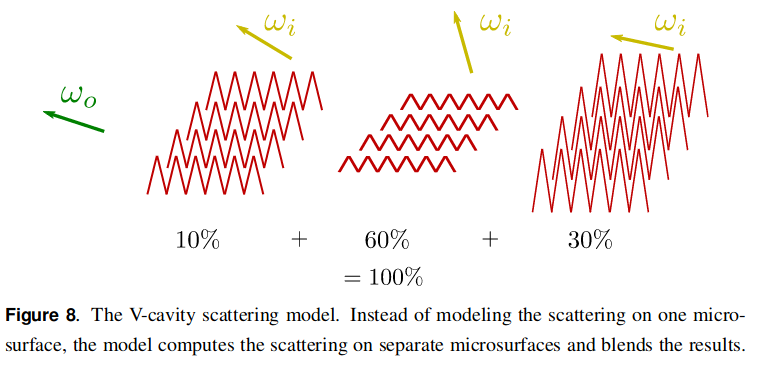
\includegraphics[width=\textwidth]{Figure8.png}
    \caption{}
    \label{fig:8}
\end{figure}

V型空洞マイクロサーフェスのmasking関数を求めるには通常三角法による導出が示される。節\ref{sec:2.3}で議論された、可視マイクロサーフェスの射影面積が保存されるという性質から、シンプルに同様の結果を導き出すことができる。V型空洞マイクロサーフェスは2つの対称的な法線$\boldsymbol{\omega}_m$と$\boldsymbol{\omega}_m'$のみを持つ。したがって、このマイクロサーフェスの法線分布は以下のようになる。

\begin{equation}
    D(\boldsymbol{\omega}) = \frac{1}{2} \frac{\delta_{\boldsymbol{\omega}_m}(\boldsymbol{\omega})}{\boldsymbol{\omega}_m \cdot \boldsymbol{\omega}_g} + \frac{1}{2} \frac{\delta_{\boldsymbol{\omega}_m'}(\boldsymbol{\omega})}{\boldsymbol{\omega}_m' \cdot \boldsymbol{\omega}_g}
    \label{eq:44}
\end{equation}

そして、以下によりこれが正しく正規化されていることを確認できる。

\begin{equation}
    \begin{split}
        \int_{\Omega} \langle \boldsymbol{\omega}, \boldsymbol{\omega}_g \rangle D(\boldsymbol{\omega}) d\boldsymbol{\omega}
        &= \int_{\Omega} \langle \boldsymbol{\omega}, \boldsymbol{\omega}_g \rangle \left( \frac{1}{2} \frac{\delta_{\boldsymbol{\omega}_m}(\boldsymbol{\omega})}{\boldsymbol{\omega}_m \cdot \boldsymbol{\omega}_g} + \frac{1}{2} \frac{\delta_{\boldsymbol{\omega}_m'}(\boldsymbol{\omega})}{\boldsymbol{\omega}_m' \cdot \boldsymbol{\omega}_g} \right) d\boldsymbol{\omega} \\
        &= \frac{1}{2} \frac{\boldsymbol{\omega}_m' \cdot \boldsymbol{\omega}_g}{\boldsymbol{\omega}_m' \cdot \boldsymbol{\omega}_g} + \frac{1}{2} \frac{\boldsymbol{\omega}_m' \cdot \boldsymbol{\omega}_g}{\boldsymbol{\omega}_m' \cdot \boldsymbol{\omega}_g} \\
        &= \frac{1}{2} + \frac{1}{2} = 1
    \end{split}
    \label{eq:45}
\end{equation}

masking項を導くため、式\eqref{eq:14}で表される可視射影面積の保存則を用いる。

\begin{equation}
    \begin{split}
        \cos\theta_o
        &= \int_{\Omega} G_1(\boldsymbol{\omega}_o, \boldsymbol{\omega}) \langle \boldsymbol{\omega}_o, \boldsymbol{\omega} \rangle D(\boldsymbol{\omega}) d\boldsymbol{\omega} \\
        &= \frac{1}{2} G_1(\boldsymbol{\omega}_o, \boldsymbol{\omega}_m) \frac{\langle \boldsymbol{\omega}_o, \boldsymbol{\omega}_m \rangle}{\boldsymbol{\omega}_m \cdot \boldsymbol{\omega}_g} + \frac{1}{2} G_1(\boldsymbol{\omega}_o, \boldsymbol{\omega}_m') \frac{\langle \boldsymbol{\omega}_o, \boldsymbol{\omega}_m' \rangle}{\boldsymbol{\omega}_m' \cdot \boldsymbol{\omega}_g}
    \end{split}
    \label{eq:46}
\end{equation}

ここでは、図\ref{fig:9}に示す通り、2つの構成(configurations)を取り得る。一方の場合では、2つの法線が可視であり遮蔽されない($G_1(\boldsymbol{\omega}_o, \boldsymbol{\omega}_m) = 1$であり$G_1(\boldsymbol{\omega}_o, \boldsymbol{\omega}_m') = 1$)。他方の場合では、$\boldsymbol{\omega}_m'$が背面を向いている($G_1(\boldsymbol{\omega}_o, \boldsymbol{\omega}_m') = 0$)。このとき以下が成り立つ。

\begin{equation}
    \cos\theta_o = \frac{1}{2}G_1(\boldsymbol{\omega}_o, \boldsymbol{\omega}_m) \frac{\langle \boldsymbol{\omega}_o, \boldsymbol{\omega}_m \rangle}{\boldsymbol{\omega}_m \cdot \boldsymbol{\omega}_g}
    \label{eq:47}
\end{equation}

これを解くと、

\begin{equation}
    \begin{split}
        G_1(\boldsymbol{\omega}_o, \boldsymbol{\omega}_m)
        &= 2 \frac{\cos\theta_o (\boldsymbol{\omega}_m \cdot \boldsymbol{\omega}_g)}{\langle \boldsymbol{\omega}_o, \boldsymbol{\omega}_m \rangle} \\
        &= 2 \frac{(\boldsymbol{\omega}_m \cdot \boldsymbol{\omega}_g) (\boldsymbol{\omega}_o \cdot \boldsymbol{\omega}_g)}{\langle \boldsymbol{\omega}_o, \boldsymbol{\omega}_m \rangle}
    \end{split}
    \label{eq:48}
\end{equation}

これら2つの構成の結果は以下の1つの定式で表すことができる。

\begin{equation}
    G_1(\boldsymbol{\omega}_o, \boldsymbol{\omega}_m) = \min \left( 1, 2 \frac{(\boldsymbol{\omega}_m \cdot \boldsymbol{\omega}_g) (\boldsymbol{\omega}_o \cdot \boldsymbol{\omega}_g)}{\langle \boldsymbol{\omega}_o, \boldsymbol{\omega}_m \rangle} \right)
    \label{eq:49}
\end{equation}

これは、CookとTorranceによって用いられるV型空洞のmasking関数としてよく知られている。

\paragraph{検証(Validation)}

このモデルが式\eqref{eq:18}を満たすか、すなわち、可視法線分布が正規化されているかどうかを確かめようと思う。まず、式\eqref{eq:16}の$G_1$を置き換える。

\begin{equation}
    D_{\boldsymbol{\omega}_o}(\boldsymbol{\omega}_m) = \min \left( 1, 2 \frac{(\boldsymbol{\omega}_m \cdot \boldsymbol{\omega}_g) (\boldsymbol{\omega}_o \cdot \boldsymbol{\omega}_g)}{\langle \boldsymbol{\omega}_o, \boldsymbol{\omega}_m \rangle} \right) \frac{\langle \boldsymbol{\omega}_o, \boldsymbol{\omega}_m \rangle D(\boldsymbol{\omega}_m)}{\cos\theta_o}
    \label{eq:50}
\end{equation}

この形式は、$min(1, -)$の項があるため、調べ辛い。しかし、V型空洞モデルとSmithのモデルの主な違いは、$\theta_o \approx \frac{\pi}{2}$となるgrazing角で発生する。つまり、grazing角では常に図\ref{fig:9}構成(a)であり、2つの法線のうち1つは背面を向いていると言える。この場合、$min(1, -)$の部分は取り除くことができる。

\begin{figure}
    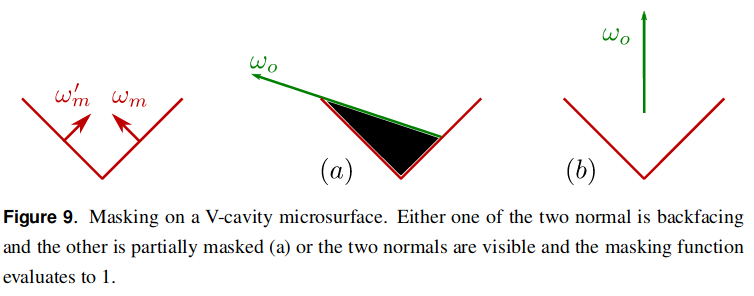
\includegraphics[width=\textwidth]{Figure9.png}
    \caption{}
    \label{fig:9}
\end{figure}

\begin{equation}
    \begin{split}
        D_{\boldsymbol{\omega}_o}(\boldsymbol{\omega}_m)
        &= 2 \frac{(\boldsymbol{\omega}_m \cdot \boldsymbol{\omega}_g) (\boldsymbol{\omega}_o \cdot \boldsymbol{\omega}_g)}{\langle \boldsymbol{\omega}_o, \boldsymbol{\omega}_m \rangle} \frac{\langle \boldsymbol{\omega}_o, \boldsymbol{\omega}_m \rangle D(\boldsymbol{\omega}_m)}{\cos\theta_o} \\
        &= 2 \chi^+(\boldsymbol{\omega}_o \cdot \boldsymbol{\omega}_m) (\boldsymbol{\omega}_m \cdot \boldsymbol{\omega}_g) D(\boldsymbol{\omega}_m) d\boldsymbol{\omega}_m
    \end{split}
    \label{eq:51}
\end{equation}

ここで、クランプされた内積$\langle \boldsymbol{\omega}_o, \boldsymbol{\omega}_m \rangle$は打ち消されるが、背面の法線が分布から取り除かれていることを保証するため、ヘヴィサイド関数$\chi^+(\boldsymbol{\omega}_o \cdot \boldsymbol{\omega}_m)$は残してあることに注意したい。この結果を以下の式を計算することで、式\eqref{eq:18}、つまり、可視法線分布が正規化されていることを検証する。

\begin{equation}
    \int_{\Omega} D_{\boldsymbol{\omega}_o}(\boldsymbol{\omega}_m) d\boldsymbol{\omega}_m = 2 \int_{\Omega} \chi^+(\boldsymbol{\omega}_o \cdot \boldsymbol{\omega}_m) (\boldsymbol{\omega}_m \cdot \boldsymbol{\omega}_g) D(\boldsymbol{\omega}_m) d\boldsymbol{\omega}_m
    \label{eq:52}
\end{equation}

grazing角では幾何学的な法線に対して出射方向がほぼ垂直になるため、ヘヴィサイド関数は分布のほぼ中央で積分を切り詰める。また、V型空洞の表面は法線分布が対称であること、つまり、$D(\boldsymbol{\omega}_m) = D(\boldsymbol{\omega}_m')$であることを暗に示している。これは、ヘヴィサイド関数が法線分布を等しい2つに切り分けることを意味する。

\begin{equation}
    \begin{split}
        \int_{\Omega} \chi^+(\boldsymbol{\omega}_o \cdot \boldsymbol{\omega}_m) (\boldsymbol{\omega}_m \cdot \boldsymbol{\omega}_g) D(\boldsymbol{\omega}_m) d\boldsymbol{\omega}_m
        &= \frac{1}{2} \int_{\Omega} (\boldsymbol{\omega}_m \cdot \boldsymbol{\omega}_g) D(\boldsymbol{\omega}_m) d\boldsymbol{\omega}_m \\
        &= \frac{1}{2}
    \end{split}
    \label{eq:53}
\end{equation}

ここで、法線分布は正規化されているので$\int_{\Omega} (\boldsymbol{\omega}_m \cdot \boldsymbol{\omega}_g) D(\boldsymbol{\omega}_m) d\boldsymbol{\omega}_m = 1$である。そして、この結果と式\eqref{eq:52}により、以下が成り立つ。

\begin{equation}
    \begin{split}
        \int_{\Omega} D_{\boldsymbol{\omega}_o}(\boldsymbol{\omega}_m) d\boldsymbol{\omega}_m
        &= 2 \int_{\Omega} \chi^+(\boldsymbol{\omega}_o \cdot \boldsymbol{\omega}_m) (\boldsymbol{\omega}_m \cdot \boldsymbol{\omega}_g) D(\boldsymbol{\omega}_m) d\boldsymbol{\omega}_m \\
        &= 2 \frac{1}{2} = 1
    \end{split}
    \label{eq:54}
\end{equation}

これは、入射角がgrazing角であるときに式\eqref{eq:51}の可視法線分布が正規化されていることを示している。さらなる技術的な導出を経ると、どの入射角でもこの分布が正規化されていることを示すことができる。

このモデルを検証する異なる方法としては、Weak White Furnaceテストがある。これを行うには、式\eqref{eq:49}の$G_1$を用いて式\eqref{eq:36}を評価する。実際には、この評価は数値積分によって行われる。この積分は常に$1$になり、したがって、V型空洞によるモデルは数学的に良く設計されており、エネルギー保存則を満たしている。

\paragraph{性質(Properties)}

V型空洞の可視法線分布が数学的にwell definedでありながらも、物理的にもっともらしい(plausible)とは言えず、入射角がgrazingのときのサーフェス・プロファイルは非現実的なモデル化が行われている。

この法線には2つの種類がある。1つは背面を向いており、ヘヴィサイド項により取り除かれる。もう1つは背面を向いておらず、$(\boldsymbol{\omega}_m \cdot \boldsymbol{\omega}_g) D(\boldsymbol{\omega}_m)$で重み付けされる放射輝度の寄与を生み出す。ここで、$(\boldsymbol{\omega}_m \cdot \boldsymbol{\omega}_g)$は、図\ref{fig:3}(a)で示されるように、マイクロファセットによる幾何学的な表面への射影のヤコビアンである。したがって、マイクロファセットは、出射方向に射影される前に幾何学的表面に射影されるかの如く、正確に重み付けされる。結果として、幾何学的に平坦なマイクロサーフェスをシミュレートしている。マイクロファセットは光の反射をかき乱す(purturb)ことができるが、幾何学的にはそのようなものは存在しない。ゆえに、このマイクロサーフェスモデルは、図\ref{fig:10}に示すように、ディスプレースメントマップではなくノーマルマップに近い振る舞いをするため、現実感が無くなってしまう。

V型空洞モデルは、1つのマイクロサーフェスをシミュレートするのではなく、法線のペアごとに1つのマイクロサーフェスをシミュレートしてその結果を平均化することから、この効果は予期されていた。1つのマイクロサーフェスならば、高確率な可視法線は低確率な可視法線より多くの射影面積を占める、すなわち、より高い寄与を生み出すと思われる。しかし、V型空洞では、異なる法線は別々にシミュレートされて法線分布によって重み付けされるため、この現象が発生しない。(背面を向いている法線が破棄されること以外は)重みに視点に対する依存性が存在しない。これが、V型空洞モデルは可視性の効果をほとんど(poorly)含まず、ノーマルマップのような何かをシミュレートするに留まっている理由である。

入射角がマイクロサーフェスすれすれ(grazing the microsurface)になればなるほど、マイクロサーフェス・プロファイルはこのノーマルマップの振る舞いをさらに強く示す傾向にある。結果として、BRDFのピークが低くなりすぎてしまうという傾向が現れる。現実のマイクロサーフェスでは、出射方向を向いている法線は、その射影面積が大きくなればなるほど、BRDFに対してより高い寄与を持つ。このため、図\ref{fig:10}に示す通り、反射方向は出射方向に変化しやすい(tend to be shifted)。この効果は、マイクロファセットは幾何学的に存在しないため、ノーマルマップにおいては見られない。つまり、法線はすべて同じ射影面積を持っている。

\begin{figure}
    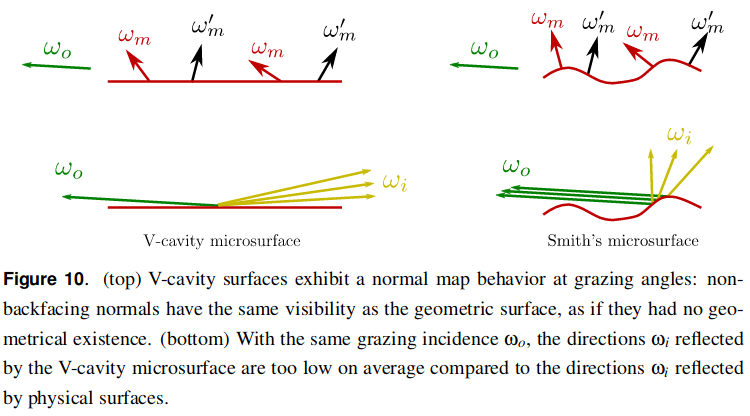
\includegraphics[width=\textwidth]{Figure10.png}
    \caption{}
    \label{fig:10}
\end{figure}

図\ref{fig:11}は、V型空洞とSmithのmasking-shadowing関数による等方的なBeckmann分布によって生成されたBRDFと、一致するGaussian statisticsを持つ手続き的な確率論的マイクロサーフェスモデルの散乱に対する数値的なシミュレーションから計算された結果を示している。Smithのmasking関数では、その分布が、ラフネスの増加に伴い、出射方向に傾いてゆく(is shifted toward)のが確認できる。非常に高いラフネス値では、BRDFでさえ後方散乱(backscattering)が主に起こる。この効果は --- 計測データ中に存在しており --- 、出射方向を向いた法線が最も多く見えることから、予期されていたことである。一方で、V型空洞モデルからはこの効果は現れない。

\begin{figure}
    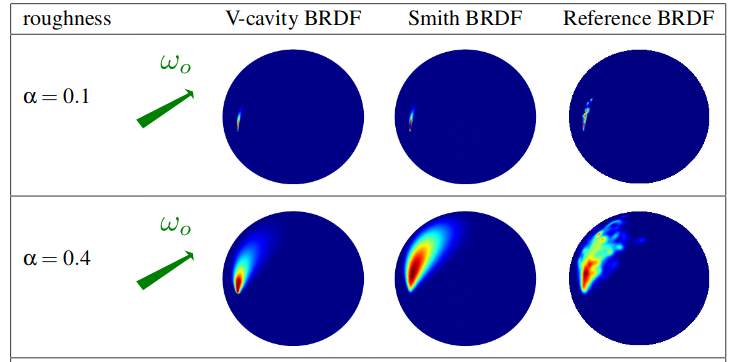
\includegraphics[width=\textwidth]{Figure11_1.png}
    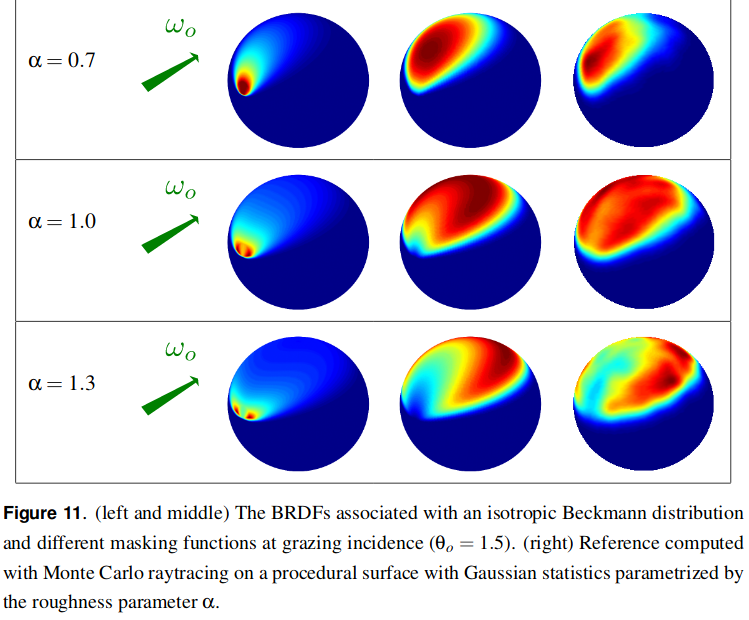
\includegraphics[width=\textwidth]{Figure11_2.png}
    \caption{}
    \label{fig:11}
\end{figure}

\subsection{非物理ベースmasking関数(Non-Physically Based Masking Functions)}

\paragraph{定義(Definition)}

マイクロサーフェスモデルから導き出された、もしくは、物理的なマイクロサーフェスを計測したものであれば、そのmasking関数は"物理ベース"と分類していたことを思い出して欲しい。物理ベースなmasking関数は常に式\eqref{eq:14}、\eqref{eq:18}、\eqref{eq:36}、\eqref{eq:37}を満たす。逆に(reciprocally)、"非物理ベース"なmasking関数はこれらの式を満たさない。すなわち、これらを導き出す(または、計測する)ことができるマイクロサーフェスが存在しないことを意味する。

\paragraph{暗黙的なmasking関数(Implicit Masking Function)}

式\eqref{eq:29}で与えられた鏡面的なマイクロファセットベースBRDFの式を簡単化するために、多くのモデルは、masking-shadowing関数と分母の式$|\boldsymbol{\omega}_g \cdot \boldsymbol{\omega}_o| |\boldsymbol{\omega}_g \cdot \boldsymbol{\omega}_i|$が互いを打ち消すと仮定して取り除かれる。つまり、masking-shadowingは暗に以下のように定義されると言える。

\begin{equation}
    G_2(\boldsymbol{\omega}_o, \boldsymbol{\omega}_i, \boldsymbol{\omega}_m) = G_1(\boldsymbol{\omega}_o, \boldsymbol{\omega}_m) G_1(\boldsymbol{\omega}_i, \boldsymbol{\omega}_m)
    \label{eq:55}
\end{equation}

ここで、分割されたmasking関数とshadowing関数は以下のようになる。

\begin{equation}
    G_1(\boldsymbol{\omega}_o, \boldsymbol{\omega}_m) = \chi^+(\boldsymbol{\omega}_o \cdot \boldsymbol{\omega}_m) \langle \boldsymbol{\omega}_o, \boldsymbol{\omega}_g \rangle
    \label{eq:56}
\end{equation}

\begin{equation}
    G_1(\boldsymbol{\omega}_i, \boldsymbol{\omega}_m) = \chi^+(\boldsymbol{\omega}_i \cdot \boldsymbol{\omega}_m) \langle \boldsymbol{\omega}_i, \boldsymbol{\omega}_g \rangle
    \label{eq:57}
\end{equation}

このmasking関数は、$\boldsymbol{\omega}_o = \boldsymbol{\omega}_g$のとき$G_1(\boldsymbol{\omega}_o, \boldsymbol{\omega}_m) = 1$であり、入射角が$\frac{\pi}{2}$に近づくに連れて$G_1(\boldsymbol{\omega}_o, \boldsymbol{\omega}_m) = 0$になるよう減少するため、"もっともらしい"と言える。しかし、このmasking関数は物理ベースではない。もちろん、式\eqref{eq:14}による射影面積の保存則を満たさない。これは、このmasking関数から導き出せる物理的なマイクロサーフェスモデルが存在しないことを示している。

\paragraph{Schlick-Smithのmasking関数(The Schlick-Smith Masking Function)}

Schlickは、しばしば"Schlick-Smith"のmasking関数として参照される、Smithのmasking関数の近似を提案した。このmasking関数には3つの問題がある。

1つ目は、その論文で使われているラフネスのパラメータ$m$に矛盾がある(inconsist)ことである。その論文の式(18)はマイクロサーフェスの二乗平均平方根(root mean square; RMS)の傾斜を指している。つまり$m$は、物理学の文献や、特にオリジナルのSmithの論文で時折使われているラフネスの記述子(descriptor)$m = \sigma$である。これは同じ式中の変数$h$の定義と一致している。しかしながら、その論文の式(20)の中だと、$m$はBeckmann分布のラフネスパラメータ$m = \alpha = \sqrt{2} \sigma$である。これは、RMSの傾斜を$\sqrt{2}$倍したものである。結果として、masking関数で使われているラフネスと法線分布で使われているラフネスに不整合が生じている。

この矛盾は容易に解決できるが、さらなる重大な(critical)問題が、彼によるSmithのmasking関数の再定式化(その論文の式(18))に誤りがあることである。彼は、"いくつかの同値(equivalences)により、オリジナルの式$G$は以下のように..."と述べている(states)。その導出は書かれていない(not provided)が、SchlickはHeらの式(その論文の式(24)と(25))を再編成された(rearranged)ように思われる。これには、Smithの$\Lambda$関数から指数の項が欠落している、というtypoが含まれている。

\begin{figure}
    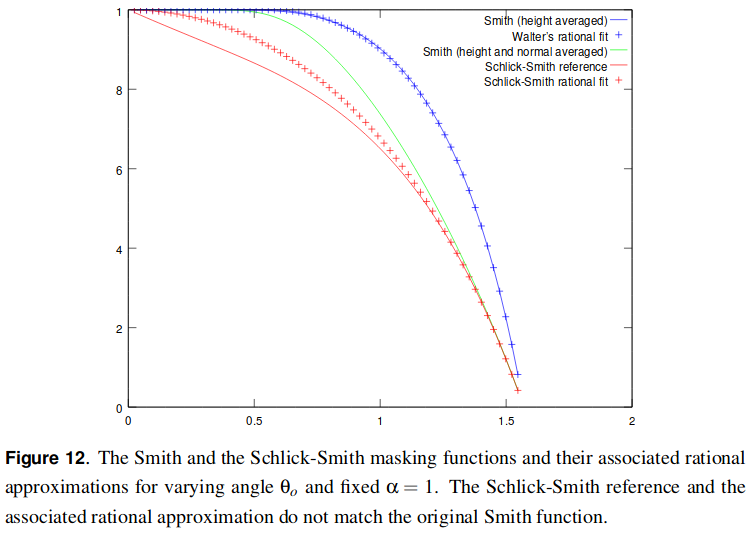
\includegraphics[width=\textwidth]{Figure12.png}
    \caption{}
    \label{fig:12}
\end{figure}

さらに、節\ref{sec:4.1}の最後のパラグラフで、幾何光学的なBRDFモデルに使うためのSmithのmasking関数はマイクロサーフェスの高さに対して平均化したものであると説明した。しかし、Schlickは、Heらの高さと法線を平均化するSmithのmasking関数を引き続き使ってしまった。これは、波動光学モデルの文脈においてなら適切であった。

2つの失敗(error)の結論としては、図\ref{fig:12}のプロットが示す通り、Schlickのオリジナルの定式もフィッティングした近似式もどちらもSmithのmasking関数に正しくマッチしない。これは"Schlick-Smith"のmasking関数が、式\ref{eq:14}から射影面積の保存則を保証できないため、物理ベースでないことを意味する。

\paragraph{Kelemenのmasking関数(The Kelemen Masking Function)}

Kelemenらは、以下の近似式を用いて、V型空洞モデルのmasking-shadowing関数と、式\eqref{eq:29}で与えられる鏡面的なマイクロファセットベースBRDFの分母を置き換える安価な方法を提案した。

\begin{equation}
    \frac{G_2(\boldsymbol{\omega}_o, \boldsymbol{\omega}_i, \boldsymbol{\omega}_h)}{|\boldsymbol{\omega}_g \cdot \boldsymbol{\omega}_o| |\boldsymbol{\omega}_g \cdot \boldsymbol{\omega}_i|} = \frac{1}{|\boldsymbol{\omega}_o \cdot \boldsymbol{\omega}_h| |\boldsymbol{\omega}_i \cdot \boldsymbol{\omega}_h|}
    \label{eq:58}
\end{equation}

これは、masking関数とshadowing関数を以下の式で近似することと等価である。

\begin{equation}
    G_1(\boldsymbol{\omega}_o, \boldsymbol{\omega}_h) = \frac{|\boldsymbol{\omega}_g \cdot \boldsymbol{\omega}_o|}{|\boldsymbol{\omega}_o \cdot \boldsymbol{\omega}_h|}
    \label{eq:59}
\end{equation}

\begin{equation}
    G_1(\boldsymbol{\omega}_i, \boldsymbol{\omega}_h) = \frac{|\boldsymbol{\omega}_g \cdot \boldsymbol{\omega}_i|}{|\boldsymbol{\omega}_i \cdot \boldsymbol{\omega}_h|}
    \label{eq:60}
\end{equation}

このmasking関数はV型空洞のmasking関数に近い。$|\boldsymbol{\omega}_g \cdot \boldsymbol{\omega}_o|$は幾何学的表面の射影面積であり、$|\boldsymbol{\omega}_o \cdot \boldsymbol{\omega}_h|$はマイクロファセットの射影面積である。つまりこの式により、マイクロファセットの射影面積が幾何学的表面の射影面積に置き換えられる。これは、ノーマルマップのように平坦なマイクロファセットのよるマイクロサーフェスをシミュレートする傾向がある。

しかし、V型空洞のmasking関数と異なり、Kelemenのmasking関数は式\eqref{eq:14}から射影面積が保存されること保証しない。これはV型空洞のmasking関数に対する良い近似であり続けるが、Kelemenの式から導出される物理的モデルは存在しない。それはすなわち、物理ベースではない。

\subsection{まとめ(Summary)}

この章では、以下を示した。

\begin{itemize}
    \item Smithのmasking関数とV型空洞のmasking関数はともに物理ベースであるが、異なるマイクロサーフェス・プロファイルを仮定している。
    \item ともに、\eqref{eq:14}から射影面積が保存することを保証する。
    \item ともに、式\eqref{eq:18}の可視法線分布の正規化係数である。
    \item ともに、式\eqref{eq:36}と\eqref{eq:37}で与えられるWeak White Furnaceテストを満足する。
    \item 対して、暗黙的masking関数、Schlick-Smithのmasking関数、Kelemenのmasking関数は式\eqref{eq:14}、\eqref{eq:18}、\eqref{eq:36}、\eqref{eq:37}を満たさない。したがって、これらは物理ベースではない。つまり、これらの式から導き出せるマイクロサーフェス・プロファイルが存在しない。
\end{itemize}

\paragraph{Smithのmasking関数(The Smith Masking Function)}

代表的な説(typical belief)のひとつに、"Smithのmasking関数は法線分布に依存しているため、良い近似である。"というものがある。我々は、この回答については正しいが、理由については間違っていることを、以下のアイデアを開発することで示した。

\begin{itemize}
    \item Smithのモデルを選択することは、可視法線の方向がmasking確率に依存しないマイクロサーフェスを仮定することを選択したと暗に示している。
    \item この仮定の下、masking関数は完全に決定される。その完全形式(exact form)は、Smithのmasking関数の一般形式として導き出すことができる。
\end{itemize}

ここでのポイントは、Smithのmasking関数を選択する理由が法線分布によってパラメータ化された物理的にもっともらしい近似だからではない、ということである。これを選ぶ本当の理由は、Smithの式が選ばれたマイクロサーフェス・プロファイル(つまり、法線/masking独立)の仮定の下では厳密な(exact)masking関数であること、である。物理的にもっともらしく、法線分布によってパラメータ化されているということは、それを選ぶ直接的な理由ではないが、正しい物理ベースmasking関数を使うことで予期される副次的効果ではある。

\paragraph{V型空洞のmasking関数(The V-Cavity Masking Function)}

もうひとつの誤解として、"V型空洞のmasking関数は、法線分布に基づかないので、間違いである。"というものがある。この章では、我々は、この推論が誤りであり、V型空洞モデルによって生み出された近似には重要な制約があることを示した。すなわち以下を示した。

\begin{itemize}
    \item 法線毎のV型空洞のmasking関数は法線分布に依存しない。
    \item しかし、V型空洞のmasking関数の平均は法線分布に依存している。これはSmithのモデルとは逆に、masking関数と法線が独立していると仮定していないためである。表面のラフネスが増加すれば、BRDFの平均遮蔽率(average masking)は増加する。
    \item V型空洞のmasking関数はいかなる対称的な法線分布でも用いることができ、正しく正規化されることが保証されている。
    \item しかし、V型空洞モデルによって仮定されるサーフェス・プロファイルは、入射角がgrazingのときに平坦なマイクロファセットを持つような、ノーマルマップのそれに近い応答を有している。
    \item grazing角や高いラフネスでは、現実の材質から予測されると比較して、BRDFのlobeが小さくなりすぎてしまう、というのが結論である。
\end{itemize}

V型空洞とSmithのどちらを選ぶかという問いには、両方ともマイクロサーフェス・プロファイルに基づいており、数学的にwell definedであることから、決定的な答えは存在しない。V型空洞は計算コストがより低く、一般的である --- 数学的にいかなる法線分布でもイケる --- が、現実感の点で劣るところがある。対して、Smithベースのモデルはより正確であるが、特定の導出と時々高価な評価が必要である。したがって、この選択は現実感とパフォーマンスのトレードオフの問題である。

\section{masking関数の伸縮不変性(Stretch Invariance of the Masking Function)}

\subsection{masking確率の不変性(Masking Probability Invariance)}

図\ref{fig:13}は、一次元の形状(configuration)を引き伸ばしたとき、与えられた出射方向に対するマイクロサーフェスのmaskingに与える影響を示している。形状を引き伸ばすことは、その画像を引き伸ばすことに等しい。すなわち、それはある次元に定数をかけることに等しい。この操作(operation)は形状のトポロジーを変化させない。つまり、伸長したあとでも、遮蔽されるレイは遮蔽されるままだし、遮蔽されないレイは遮蔽されないままである。これは重要な(key)性質である。すなわち、形状に含まれるすべての傾斜が同時にスケールするとき、masking確率は形状の伸長に対して不変である。これにはマイクロサーフェスの傾斜も含まれ、その傾斜は出射方向に関係づけられている。これらはすべて伸長ファクタの逆数でスケールする。したがって、傾斜分布(the distribution of slopes)の幅は伸長ファクタの逆数で伸長する。

\begin{figure}
    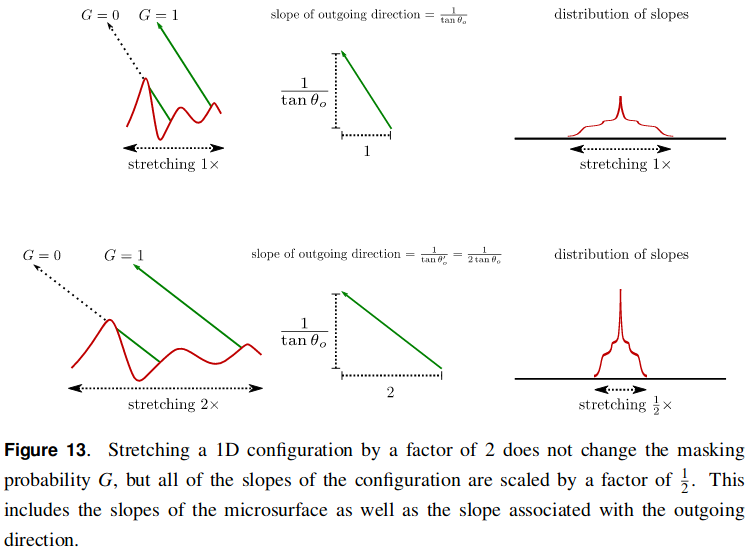
\includegraphics[width=\textwidth]{Figure13.png}
    \caption{}
    \label{fig:13}
\end{figure}

\subsection{傾斜分布(The Distribution of Slopes)}

マイクロサーフェスが高さフィールド(hightfield)であるならば、マイクロサーフェスの高さの分布はよく$P^1(h)$で示される。このときのマイクロサーフェスの傾斜は高さの勾配$(x_{\tilde{m}}, y_{\tilde{m}}) = \nabla h$で示される。つまり、マイクロサーフェスの高さが空間的にどれだけ変化しているかを計測することを表している。マイクロサーフェスの傾斜分布は$P^{22}(x_{\tilde{m}}, y_{\tilde{m}})$で示される。ここで、$\tilde{m} = (x_{\tilde{m}}, y_{\tilde{m}})$は法線$\boldsymbol{\omega}_m = (x_m, y_m, z_m)$に関連する傾斜であり、以下で表される。

\begin{equation}
    \tilde{m} = (x_{\tilde{m}}, y_{\tilde{m}}) = (-\frac{x_m}{z_m}, -\frac{y_m}{z_m}) = -\tan\theta_m(\cos\phi_m, \sin\phi_m)
    \label{eq:61}
\end{equation}

逆に考えると、$\omega_m$は以下で表される。

\begin{equation}
    \omega_m = \frac{(-x_{\tilde{m}}, -y_{\tilde{m}}, 1)}{\sqrt{x_{\tilde{m}}^2 + y_{\tilde{m}}^2 + 1}}
    \label{eq:62}
\end{equation}

傾斜分布は正規化されている必要がある。

\begin{equation}
    \int_{-\infty}^{\infty} \int_{-\infty}^{\infty} P^{22}(x_{\tilde{m}}, y_{\tilde{m}}) dx_{\tilde{m}} dy_{\tilde{m}} = 1
    \label{eq:63}
\end{equation}

傾斜分布から法線分布を作ることができる。

\begin{equation}
    D(\omega_m) = \frac{P^{22}(x_{\tilde{m}}, y_{\tilde{m}})}{\cos^{4} \theta_m}
    \label{eq:64}
\end{equation}

ラフネスパラメータが明示されなければならないならば、等方的な分布には$D(\omega_m, \alpha)$と$P^{22}(x_{\tilde{m}}, y_{\tilde{m}}, \alpha)$の表記を、異方的な分布には$D(\omega_m, \alpha_x, \alpha_y)$と$P^{22}(x_{\tilde{m}}, y_{\tilde{m}}, \alpha_x, \alpha_y)$の表記を使う。

\subsection{等方的な形状不変の傾斜分布(Isotropic Shape-Invariant Distributions of Slopes)}

\paragraph{形状不変(Shape-Invariance)}

いくつかの等方的なパラメータを持つ(parametric)傾斜分布$P^{22}$はラフネスパラメータ$\alpha$に依存する。このとき、$\alpha$を変化させることは形(shape)を変化させずに分布を伸長することと等価である。これは、傾斜分布が、角度$\theta_m$の法線における傾斜の大きさ(amplitude)$\tan\theta_m = \sqrt{x_{\tilde{m}}^2 + y_{\tilde{m}}^2}$とラフネスパラメータ$\alpha$との割合$\frac{\tan\theta_m}{\alpha}$にのみ依存する場合であり、以下で表される。

\begin{equation}
    P^{22}(x_{\tilde{m}}, y_{\tilde{m}}, \alpha) = \frac{1}{\alpha_2} f \left( \frac{\sqrt{x_{\tilde{m}}^2 + y_{\tilde{m}}^2}}{\alpha} \right) = \frac{1}{\alpha^2} f \left( \frac{\tan\theta_m}{\alpha} \right)
    \label{eq:65}
\end{equation}

ここで、$f$は分布の形を定義する一次元の関数である。これらの傾斜分布は\textbf{形状不変(shape-invariant)}という。それは、この性質が示される分布は常に同じ形$f$を持ち、ラフネスパラメータによってのみ引き伸ばされ、スケールされるためである。つまり、以下で表される。

\begin{equation}
    P^{22}(x_{\tilde{m}}, y_{\tilde{m}}, \alpha) = \frac{1}{\lambda^2} P^{22}(\frac{x_{\tilde{m}}}{\lambda}, \frac{y_{\tilde{m}}}{\lambda}, \frac{\alpha}{\lambda}) \text{, for any } \lambda > 0
    \label{eq:66}
\end{equation}

図\ref{fig:13}で示した通り、等方的な形状不変の傾斜分布において、その形状(configuration)を伸長することは、ラフネスパラメータ$\alpha$と出射ベクトルの傾斜を同じファクタでスケールさせることと等価である。これはmasking関数が変数$a = \frac{1}{\alpha\tan\theta_o}$にのみ依存することを暗に示している。ここで、$\frac{1}{\tan\theta_o}$は出射方向の傾斜を表す。...

TODO

\appendix

\section{(Derivation of the Masking Function)}
\label{sec:A}

\end{document}
